\documentclass[twoside]{book}

% Packages required by doxygen
\usepackage{fixltx2e}
\usepackage{calc}
\usepackage{doxygen}
\usepackage[export]{adjustbox} % also loads graphicx
\usepackage{graphicx}
\usepackage[utf8]{inputenc}
\usepackage{makeidx}
\usepackage{multicol}
\usepackage{multirow}
\PassOptionsToPackage{warn}{textcomp}
\usepackage{textcomp}
\usepackage[nointegrals]{wasysym}
\usepackage[table]{xcolor}

% Font selection
\usepackage[T1]{fontenc}
\usepackage[scaled=.90]{helvet}
\usepackage{courier}
\usepackage{amssymb}
\usepackage{sectsty}
\renewcommand{\familydefault}{\sfdefault}
\allsectionsfont{%
  \fontseries{bc}\selectfont%
  \color{darkgray}%
}
\renewcommand{\DoxyLabelFont}{%
  \fontseries{bc}\selectfont%
  \color{darkgray}%
}
\newcommand{\+}{\discretionary{\mbox{\scriptsize$\hookleftarrow$}}{}{}}

% Page & text layout
\usepackage{geometry}
\geometry{%
  a4paper,%
  top=2.5cm,%
  bottom=2.5cm,%
  left=2.5cm,%
  right=2.5cm%
}
\tolerance=750
\hfuzz=15pt
\hbadness=750
\setlength{\emergencystretch}{15pt}
\setlength{\parindent}{0cm}
\setlength{\parskip}{3ex plus 2ex minus 2ex}
\makeatletter
\renewcommand{\paragraph}{%
  \@startsection{paragraph}{4}{0ex}{-1.0ex}{1.0ex}{%
    \normalfont\normalsize\bfseries\SS@parafont%
  }%
}
\renewcommand{\subparagraph}{%
  \@startsection{subparagraph}{5}{0ex}{-1.0ex}{1.0ex}{%
    \normalfont\normalsize\bfseries\SS@subparafont%
  }%
}
\makeatother

% Headers & footers
\usepackage{fancyhdr}
\pagestyle{fancyplain}
\fancyhead[LE]{\fancyplain{}{\bfseries\thepage}}
\fancyhead[CE]{\fancyplain{}{}}
\fancyhead[RE]{\fancyplain{}{\bfseries\leftmark}}
\fancyhead[LO]{\fancyplain{}{\bfseries\rightmark}}
\fancyhead[CO]{\fancyplain{}{}}
\fancyhead[RO]{\fancyplain{}{\bfseries\thepage}}
\fancyfoot[LE]{\fancyplain{}{}}
\fancyfoot[CE]{\fancyplain{}{}}
\fancyfoot[RE]{\fancyplain{}{\bfseries\scriptsize Generated by Doxygen }}
\fancyfoot[LO]{\fancyplain{}{\bfseries\scriptsize Generated by Doxygen }}
\fancyfoot[CO]{\fancyplain{}{}}
\fancyfoot[RO]{\fancyplain{}{}}
\renewcommand{\footrulewidth}{0.4pt}
\renewcommand{\chaptermark}[1]{%
  \markboth{#1}{}%
}
\renewcommand{\sectionmark}[1]{%
  \markright{\thesection\ #1}%
}

% Indices & bibliography
\usepackage{natbib}
\usepackage[titles]{tocloft}
\setcounter{tocdepth}{3}
\setcounter{secnumdepth}{5}
\makeindex

% Hyperlinks (required, but should be loaded last)
\usepackage{ifpdf}
\ifpdf
  \usepackage[pdftex,pagebackref=true]{hyperref}
\else
  \usepackage[ps2pdf,pagebackref=true]{hyperref}
\fi
\hypersetup{%
  colorlinks=true,%
  linkcolor=blue,%
  citecolor=blue,%
  unicode%
}

% Custom commands
\newcommand{\clearemptydoublepage}{%
  \newpage{\pagestyle{empty}\cleardoublepage}%
}

\usepackage{caption}
\captionsetup{labelsep=space,justification=centering,font={bf},singlelinecheck=off,skip=4pt,position=top}

%===== C O N T E N T S =====

\begin{document}

% Titlepage & ToC
\hypersetup{pageanchor=false,
             bookmarksnumbered=true,
             pdfencoding=unicode
            }
\pagenumbering{alph}
\begin{titlepage}
\vspace*{7cm}
\begin{center}%
{\Large media\+FW }\\
\vspace*{1cm}
{\large Generated by Doxygen 1.8.13}\\
\end{center}
\end{titlepage}
\clearemptydoublepage
\pagenumbering{roman}
\tableofcontents
\clearemptydoublepage
\pagenumbering{arabic}
\hypersetup{pageanchor=true}

%--- Begin generated contents ---
\chapter{Module Index}
\section{Modules}
Here is a list of all modules\+:\begin{DoxyCompactList}
\item \contentsline{section}{Queue\+Request\+Op}{\pageref{group__QueueRequestOp}}{}
\end{DoxyCompactList}

\chapter{Hierarchical Index}
\section{Class Hierarchy}
This inheritance list is sorted roughly, but not completely, alphabetically\+:\begin{DoxyCompactList}
\item \contentsline{section}{Json\+:\+:Char\+Reader}{\pageref{classJson_1_1CharReader}}{}
\begin{DoxyCompactList}
\item \contentsline{section}{Json\+:\+:Our\+Char\+Reader}{\pageref{classJson_1_1OurCharReader}}{}
\end{DoxyCompactList}
\item \contentsline{section}{Cli}{\pageref{classCli}}{}
\item \contentsline{section}{Client}{\pageref{classClient}}{}
\item \contentsline{section}{Json\+:\+:Value\+:\+:Comment\+Info}{\pageref{structJson_1_1Value_1_1CommentInfo}}{}
\item \contentsline{section}{Json\+:\+:Comment\+Style}{\pageref{structJson_1_1CommentStyle}}{}
\item \contentsline{section}{Connection}{\pageref{classConnection}}{}
\item \contentsline{section}{Json\+:\+:Value\+:\+:C\+Z\+String}{\pageref{classJson_1_1Value_1_1CZString}}{}
\item \contentsline{section}{Database}{\pageref{classDatabase}}{}
\begin{DoxyCompactList}
\item \contentsline{section}{Movie\+Database}{\pageref{classMovieDatabase}}{}
\end{DoxyCompactList}
\item \contentsline{section}{Database\+Item}{\pageref{classDatabaseItem}}{}
\item \contentsline{section}{Json\+:\+:Our\+Reader\+:\+:Error\+Info}{\pageref{classJson_1_1OurReader_1_1ErrorInfo}}{}
\item \contentsline{section}{Json\+:\+:Reader\+:\+:Error\+Info}{\pageref{classJson_1_1Reader_1_1ErrorInfo}}{}
\item std\+:\+:exception\begin{DoxyCompactList}
\item \contentsline{section}{Json\+:\+:Exception}{\pageref{classJson_1_1Exception}}{}
\begin{DoxyCompactList}
\item \contentsline{section}{Json\+:\+:Logic\+Error}{\pageref{classJson_1_1LogicError}}{}
\item \contentsline{section}{Json\+:\+:Runtime\+Error}{\pageref{classJson_1_1RuntimeError}}{}
\end{DoxyCompactList}
\end{DoxyCompactList}
\item \contentsline{section}{Json\+:\+:Char\+Reader\+:\+:Factory}{\pageref{classJson_1_1CharReader_1_1Factory}}{}
\begin{DoxyCompactList}
\item \contentsline{section}{Json\+:\+:Char\+Reader\+Builder}{\pageref{classJson_1_1CharReaderBuilder}}{}
\end{DoxyCompactList}
\item \contentsline{section}{Json\+:\+:Stream\+Writer\+:\+:Factory}{\pageref{classJson_1_1StreamWriter_1_1Factory}}{}
\begin{DoxyCompactList}
\item \contentsline{section}{Json\+:\+:Stream\+Writer\+Builder}{\pageref{classJson_1_1StreamWriterBuilder}}{}
\end{DoxyCompactList}
\item \contentsline{section}{Json\+:\+:Features}{\pageref{classJson_1_1Features}}{}
\item \contentsline{section}{Json\+Parser}{\pageref{classJsonParser}}{}
\item \contentsline{section}{Json\+:\+:Our\+Features}{\pageref{classJson_1_1OurFeatures}}{}
\item \contentsline{section}{Json\+:\+:Our\+Reader}{\pageref{classJson_1_1OurReader}}{}
\item \contentsline{section}{Json\+:\+:Path}{\pageref{classJson_1_1Path}}{}
\item \contentsline{section}{Json\+:\+:Path\+Argument}{\pageref{classJson_1_1PathArgument}}{}
\item \contentsline{section}{Json\+:\+:Reader}{\pageref{classJson_1_1Reader}}{}
\item \contentsline{section}{Json\+:\+:Static\+String}{\pageref{classJson_1_1StaticString}}{}
\item \contentsline{section}{Json\+:\+:Stream\+Writer}{\pageref{classJson_1_1StreamWriter}}{}
\begin{DoxyCompactList}
\item \contentsline{section}{Json\+:\+:Built\+Styled\+Stream\+Writer}{\pageref{structJson_1_1BuiltStyledStreamWriter}}{}
\end{DoxyCompactList}
\item \contentsline{section}{Json\+:\+:Value\+:\+:C\+Z\+String\+:\+:String\+Storage}{\pageref{structJson_1_1Value_1_1CZString_1_1StringStorage}}{}
\item \contentsline{section}{Json\+:\+:Our\+Reader\+:\+:Structured\+Error}{\pageref{structJson_1_1OurReader_1_1StructuredError}}{}
\item \contentsline{section}{Json\+:\+:Reader\+:\+:Structured\+Error}{\pageref{structJson_1_1Reader_1_1StructuredError}}{}
\item \contentsline{section}{Tags}{\pageref{structTags}}{}
\item \contentsline{section}{Json\+:\+:Our\+Reader\+:\+:Token}{\pageref{classJson_1_1OurReader_1_1Token}}{}
\item \contentsline{section}{Json\+:\+:Reader\+:\+:Token}{\pageref{classJson_1_1Reader_1_1Token}}{}
\item \contentsline{section}{Json\+:\+:Value}{\pageref{classJson_1_1Value}}{}
\item \contentsline{section}{Json\+:\+:Value\+:\+:Value\+Holder}{\pageref{unionJson_1_1Value_1_1ValueHolder}}{}
\item \contentsline{section}{Json\+:\+:Value\+Iterator\+Base}{\pageref{classJson_1_1ValueIteratorBase}}{}
\begin{DoxyCompactList}
\item \contentsline{section}{Json\+:\+:Value\+Const\+Iterator}{\pageref{classJson_1_1ValueConstIterator}}{}
\item \contentsline{section}{Json\+:\+:Value\+Iterator}{\pageref{classJson_1_1ValueIterator}}{}
\end{DoxyCompactList}
\end{DoxyCompactList}

\chapter{Class Index}
\section{Class List}
Here are the classes, structs, unions and interfaces with brief descriptions\+:\begin{DoxyCompactList}
\item\contentsline{section}{\hyperlink{structJson_1_1BuiltStyledStreamWriter}{Json\+::\+Built\+Styled\+Stream\+Writer} }{\pageref{structJson_1_1BuiltStyledStreamWriter}}{}
\item\contentsline{section}{\hyperlink{classJson_1_1CharReader}{Json\+::\+Char\+Reader} }{\pageref{classJson_1_1CharReader}}{}
\item\contentsline{section}{\hyperlink{classJson_1_1CharReaderBuilder}{Json\+::\+Char\+Reader\+Builder} \\*Build a \hyperlink{classJson_1_1CharReader}{Char\+Reader} implementation }{\pageref{classJson_1_1CharReaderBuilder}}{}
\item\contentsline{section}{\hyperlink{classCli}{Cli} \\*Class implementing the functionality of a command line interface }{\pageref{classCli}}{}
\item\contentsline{section}{\hyperlink{classClient}{Client} \\*Class implementing the functionality of a client }{\pageref{classClient}}{}
\item\contentsline{section}{\hyperlink{structJson_1_1Value_1_1CommentInfo}{Json\+::\+Value\+::\+Comment\+Info} }{\pageref{structJson_1_1Value_1_1CommentInfo}}{}
\item\contentsline{section}{\hyperlink{structJson_1_1CommentStyle}{Json\+::\+Comment\+Style} \\*Scoped enums are not available until C++11 }{\pageref{structJson_1_1CommentStyle}}{}
\item\contentsline{section}{\hyperlink{classConnection}{Connection} }{\pageref{classConnection}}{}
\item\contentsline{section}{\hyperlink{classJson_1_1Value_1_1CZString}{Json\+::\+Value\+::\+C\+Z\+String} }{\pageref{classJson_1_1Value_1_1CZString}}{}
\item\contentsline{section}{\hyperlink{classDatabase}{Database} \\*}{\pageref{classDatabase}}{}
\item\contentsline{section}{\hyperlink{classDatabaseItem}{Database\+Item} }{\pageref{classDatabaseItem}}{}
\item\contentsline{section}{\hyperlink{classJson_1_1OurReader_1_1ErrorInfo}{Json\+::\+Our\+Reader\+::\+Error\+Info} }{\pageref{classJson_1_1OurReader_1_1ErrorInfo}}{}
\item\contentsline{section}{\hyperlink{classJson_1_1Reader_1_1ErrorInfo}{Json\+::\+Reader\+::\+Error\+Info} }{\pageref{classJson_1_1Reader_1_1ErrorInfo}}{}
\item\contentsline{section}{\hyperlink{classJson_1_1Exception}{Json\+::\+Exception} }{\pageref{classJson_1_1Exception}}{}
\item\contentsline{section}{\hyperlink{classJson_1_1CharReader_1_1Factory}{Json\+::\+Char\+Reader\+::\+Factory} }{\pageref{classJson_1_1CharReader_1_1Factory}}{}
\item\contentsline{section}{\hyperlink{classJson_1_1StreamWriter_1_1Factory}{Json\+::\+Stream\+Writer\+::\+Factory} \\*A simple abstract factory }{\pageref{classJson_1_1StreamWriter_1_1Factory}}{}
\item\contentsline{section}{\hyperlink{classJson_1_1Features}{Json\+::\+Features} \\*Configuration passed to reader and writer. This configuration object can be used to force the \hyperlink{classJson_1_1Reader}{Reader} or Writer to behave in a standard conforming way }{\pageref{classJson_1_1Features}}{}
\item\contentsline{section}{\hyperlink{classJsonParser}{Json\+Parser} }{\pageref{classJsonParser}}{}
\item\contentsline{section}{\hyperlink{classJson_1_1LogicError}{Json\+::\+Logic\+Error} }{\pageref{classJson_1_1LogicError}}{}
\item\contentsline{section}{\hyperlink{classMovieDatabase}{Movie\+Database} \\*A module that implements the functionality of \hyperlink{Database_8h_source}{Database.\+h} and helps the client to perform database actions. }{\pageref{classMovieDatabase}}{}
\item\contentsline{section}{\hyperlink{classJson_1_1OurCharReader}{Json\+::\+Our\+Char\+Reader} }{\pageref{classJson_1_1OurCharReader}}{}
\item\contentsline{section}{\hyperlink{classJson_1_1OurFeatures}{Json\+::\+Our\+Features} }{\pageref{classJson_1_1OurFeatures}}{}
\item\contentsline{section}{\hyperlink{classJson_1_1OurReader}{Json\+::\+Our\+Reader} }{\pageref{classJson_1_1OurReader}}{}
\item\contentsline{section}{\hyperlink{classJson_1_1Path}{Json\+::\+Path} \\*Experimental and untested\+: represents a \char`\"{}path\char`\"{} to access a node }{\pageref{classJson_1_1Path}}{}
\item\contentsline{section}{\hyperlink{classJson_1_1PathArgument}{Json\+::\+Path\+Argument} \\*Experimental and untested\+: represents an element of the \char`\"{}path\char`\"{} to access a node }{\pageref{classJson_1_1PathArgument}}{}
\item\contentsline{section}{\hyperlink{classJson_1_1Reader}{Json\+::\+Reader} \\*Unserialize a \href{http://www.json.org}{\tt J\+S\+ON} document into a \hyperlink{classJson_1_1Value}{Value} }{\pageref{classJson_1_1Reader}}{}
\item\contentsline{section}{\hyperlink{classJson_1_1RuntimeError}{Json\+::\+Runtime\+Error} }{\pageref{classJson_1_1RuntimeError}}{}
\item\contentsline{section}{\hyperlink{classJson_1_1StaticString}{Json\+::\+Static\+String} \\*Lightweight wrapper to tag static string }{\pageref{classJson_1_1StaticString}}{}
\item\contentsline{section}{\hyperlink{classJson_1_1StreamWriter}{Json\+::\+Stream\+Writer} }{\pageref{classJson_1_1StreamWriter}}{}
\item\contentsline{section}{\hyperlink{classJson_1_1StreamWriterBuilder}{Json\+::\+Stream\+Writer\+Builder} \\*Build a \hyperlink{classJson_1_1StreamWriter}{Stream\+Writer} implementation }{\pageref{classJson_1_1StreamWriterBuilder}}{}
\item\contentsline{section}{\hyperlink{structJson_1_1Value_1_1CZString_1_1StringStorage}{Json\+::\+Value\+::\+C\+Z\+String\+::\+String\+Storage} }{\pageref{structJson_1_1Value_1_1CZString_1_1StringStorage}}{}
\item\contentsline{section}{\hyperlink{structJson_1_1OurReader_1_1StructuredError}{Json\+::\+Our\+Reader\+::\+Structured\+Error} }{\pageref{structJson_1_1OurReader_1_1StructuredError}}{}
\item\contentsline{section}{\hyperlink{structJson_1_1Reader_1_1StructuredError}{Json\+::\+Reader\+::\+Structured\+Error} \\*An error tagged with where in the J\+S\+ON text it was encountered }{\pageref{structJson_1_1Reader_1_1StructuredError}}{}
\item\contentsline{section}{\hyperlink{structTags}{Tags} \\*A module representing the content of a database item. }{\pageref{structTags}}{}
\item\contentsline{section}{\hyperlink{classJson_1_1OurReader_1_1Token}{Json\+::\+Our\+Reader\+::\+Token} }{\pageref{classJson_1_1OurReader_1_1Token}}{}
\item\contentsline{section}{\hyperlink{classJson_1_1Reader_1_1Token}{Json\+::\+Reader\+::\+Token} }{\pageref{classJson_1_1Reader_1_1Token}}{}
\item\contentsline{section}{\hyperlink{classJson_1_1Value}{Json\+::\+Value} \\*Represents a \href{http://www.json.org}{\tt J\+S\+ON} value }{\pageref{classJson_1_1Value}}{}
\item\contentsline{section}{\hyperlink{classJson_1_1ValueConstIterator}{Json\+::\+Value\+Const\+Iterator} \\*Const iterator for object and array value }{\pageref{classJson_1_1ValueConstIterator}}{}
\item\contentsline{section}{\hyperlink{unionJson_1_1Value_1_1ValueHolder}{Json\+::\+Value\+::\+Value\+Holder} }{\pageref{unionJson_1_1Value_1_1ValueHolder}}{}
\item\contentsline{section}{\hyperlink{classJson_1_1ValueIterator}{Json\+::\+Value\+Iterator} \\*Iterator for object and array value }{\pageref{classJson_1_1ValueIterator}}{}
\item\contentsline{section}{\hyperlink{classJson_1_1ValueIteratorBase}{Json\+::\+Value\+Iterator\+Base} \\*Base class for \hyperlink{classJson_1_1Value}{Value} iterators }{\pageref{classJson_1_1ValueIteratorBase}}{}
\end{DoxyCompactList}

\chapter{Module Documentation}
\hypertarget{group__QueueRequestOp}{}\section{Queue\+Request\+Op}
\label{group__QueueRequestOp}\index{Queue\+Request\+Op@{Queue\+Request\+Op}}


push incoming request to queue  


push incoming request to queue 

pop requests from queue

push\+Request 
\begin{DoxyParams}{Parameters}
{\em m\+\_\+request} & incoming request about to be queued\\
\hline
\end{DoxyParams}
pop\+Request \begin{DoxyReturn}{Returns}
popped request ready to process 
\end{DoxyReturn}

\chapter{Class Documentation}
\hypertarget{classCli}{}\section{Cli Class Reference}
\label{classCli}\index{Cli@{Cli}}


Module handling everything related to our Command line interface.  




{\ttfamily \#include \char`\"{}inc/\+Cli.\+h\char`\"{}}



Inheritance diagram for Cli\+:\nopagebreak
\begin{figure}[H]
\begin{center}
\leavevmode
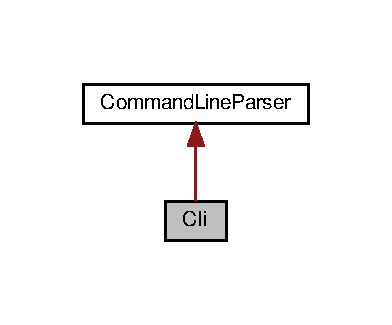
\includegraphics[width=188pt]{classCli__inherit__graph}
\end{center}
\end{figure}


Collaboration diagram for Cli\+:\nopagebreak
\begin{figure}[H]
\begin{center}
\leavevmode
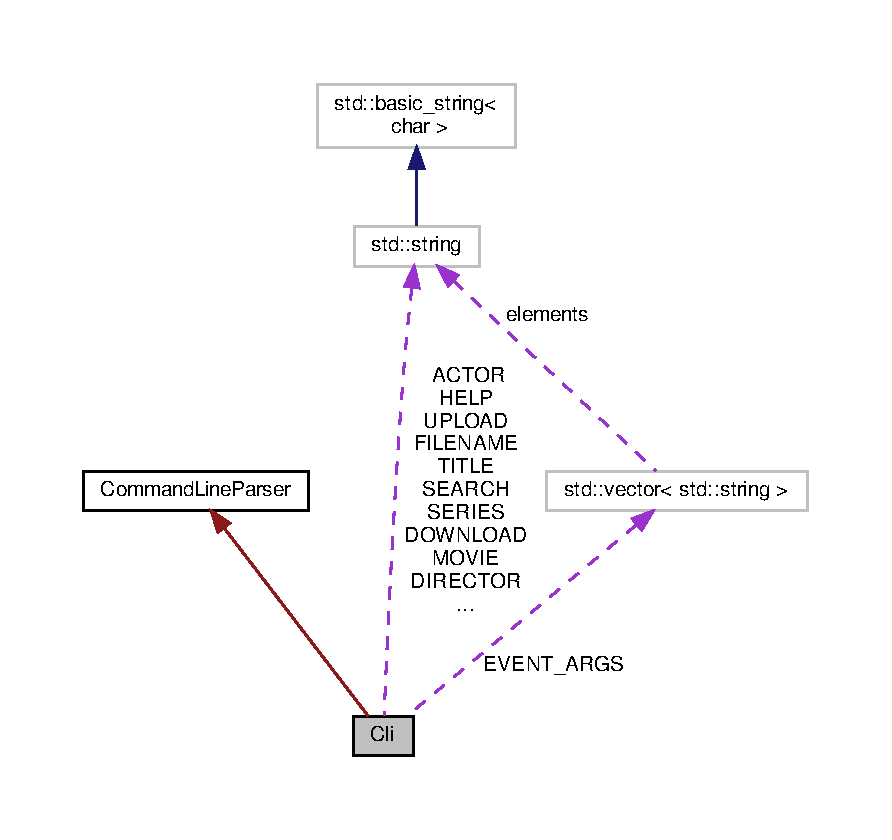
\includegraphics[width=350pt]{classCli__coll__graph}
\end{center}
\end{figure}
\subsection*{Public Member Functions}
\begin{DoxyCompactItemize}
\item 
\hyperlink{classRequest}{Request} \hyperlink{classCli_aa2b3675ef3e3bb01ed0d1997460a0e28}{process} () override
\begin{DoxyCompactList}\small\item\em Public method processing input from stdin. . \end{DoxyCompactList}\item 
\hyperlink{classRequest}{Request} \hyperlink{classCli_af29a5d8a0c3863f69c0e21133dee2d1b}{interprete} (std\+::vector$<$ std\+::string $>$ \&) override
\begin{DoxyCompactList}\small\item\em translate incoming user request and save in request object \end{DoxyCompactList}\item 
\hyperlink{classRequest}{Request} \hyperlink{classCli_a4ee41556f8c3a736d813f0d937413da0}{process} (std\+::string \&) override
\begin{DoxyCompactList}\small\item\em Public method processing input from stdin. \end{DoxyCompactList}\item 
\mbox{\Hypertarget{classCli_af21370e0e274a657bf2c9efceb18b6b3}\label{classCli_af21370e0e274a657bf2c9efceb18b6b3}} 
void {\bfseries verify\+Upload\+Test} (\hyperlink{classRequest}{Request} \&request, std\+::vector$<$ std\+::string $>$ \&i)
\end{DoxyCompactItemize}
\subsection*{Private Member Functions}
\begin{DoxyCompactItemize}
\item 
std\+::vector$<$ std\+::string $>$ \hyperlink{classCli_aaf60768f062a6dc2557aaddbe738a19c}{split} (std\+::string \&input, char delim)
\item 
\mbox{\Hypertarget{classCli_a8b6ecb803833139fc7dbdb1bac9cb127}\label{classCli_a8b6ecb803833139fc7dbdb1bac9cb127}} 
int {\bfseries check\+Valid\+Event} (std\+::vector$<$ std\+::string $>$ \&input, Event \&event)
\item 
\mbox{\Hypertarget{classCli_a116a3c89cbb5f9b807661123ee0dd5a3}\label{classCli_a116a3c89cbb5f9b807661123ee0dd5a3}} 
int {\bfseries check\+Valid\+Category} (std\+::vector$<$ std\+::string $>$ \&input, Category \&category)
\item 
\mbox{\Hypertarget{classCli_a5137618fd0eeaa34964b175aff8061ef}\label{classCli_a5137618fd0eeaa34964b175aff8061ef}} 
int {\bfseries check\+Valid\+Type} (\hyperlink{classRequest}{Request} \&request, std\+::string \&type)
\item 
\mbox{\Hypertarget{classCli_af10df67ce26c8a773e573323c47d9781}\label{classCli_af10df67ce26c8a773e573323c47d9781}} 
int {\bfseries verify\+Object\+Exists} (Category \&category, const std\+::string \&value)
\item 
\mbox{\Hypertarget{classCli_a6121ca606d1ae7b8b8b57d31786d2e18}\label{classCli_a6121ca606d1ae7b8b8b57d31786d2e18}} 
int {\bfseries get\+Type\+Of\+Value} (std\+::vector$<$ std\+::string $>$ \&input, std\+::string \&type)
\item 
\mbox{\Hypertarget{classCli_ac00196cbc1bd9683127923b13de9cbbc}\label{classCli_ac00196cbc1bd9683127923b13de9cbbc}} 
int {\bfseries get\+Value\+Of\+Type} (std\+::vector$<$ std\+::string $>$ \&input, std\+::string \&val)
\item 
\mbox{\Hypertarget{classCli_a2e2d57f7175aa6423db2a616098a3b2e}\label{classCli_a2e2d57f7175aa6423db2a616098a3b2e}} 
void {\bfseries set\+File\+Name} (\hyperlink{classRequest}{Request} \&request, std\+::string \&val)
\item 
\mbox{\Hypertarget{classCli_a0cf3263bf644c151d59b8957746a9507}\label{classCli_a0cf3263bf644c151d59b8957746a9507}} 
void {\bfseries set\+Properties} (\hyperlink{classRequest}{Request} \&request, std\+::vector$<$ std\+::string $>$ \&item)
\item 
\mbox{\Hypertarget{classCli_ae51022f0ca5e385ebd2551021f653b97}\label{classCli_ae51022f0ca5e385ebd2551021f653b97}} 
int {\bfseries verify\+Upload} (\hyperlink{classRequest}{Request} \&request)
\item 
void \hyperlink{classCli_a8251d6c89698aaf128318fc3ad4b2906}{print\+Options} ()
\begin{DoxyCompactList}\small\item\em Test A private method that prints all valid options for stdin. \end{DoxyCompactList}\end{DoxyCompactItemize}
\subsection*{Private Attributes}
\begin{DoxyCompactItemize}
\item 
\mbox{\Hypertarget{classCli_a6b39501d775b2719cdacd6937507906a}\label{classCli_a6b39501d775b2719cdacd6937507906a}} 
const std\+::string {\bfseries T\+I\+T\+LE} = \char`\"{}title\char`\"{}
\item 
\mbox{\Hypertarget{classCli_ae49ac3e6fb12dfa20c41ca189cbcd863}\label{classCli_ae49ac3e6fb12dfa20c41ca189cbcd863}} 
const std\+::string {\bfseries G\+E\+N\+RE} = \char`\"{}genre\char`\"{}
\item 
\mbox{\Hypertarget{classCli_af1bfe00ff8a3f8415e74b39970007f1b}\label{classCli_af1bfe00ff8a3f8415e74b39970007f1b}} 
const std\+::string {\bfseries A\+C\+T\+OR} = \char`\"{}actor\char`\"{}
\item 
\mbox{\Hypertarget{classCli_ae1510a4c9ae1696862bf6362eddfdb63}\label{classCli_ae1510a4c9ae1696862bf6362eddfdb63}} 
const std\+::string {\bfseries D\+I\+R\+E\+C\+T\+OR} = \char`\"{}director\char`\"{}
\item 
\mbox{\Hypertarget{classCli_a25d22c371e6d1a701a375dd77b98a839}\label{classCli_a25d22c371e6d1a701a375dd77b98a839}} 
const std\+::string {\bfseries F\+I\+L\+E\+N\+A\+ME} = \char`\"{}filename\char`\"{}
\item 
\mbox{\Hypertarget{classCli_a74a219ff6c475389cbcffaeaad0f0315}\label{classCli_a74a219ff6c475389cbcffaeaad0f0315}} 
std\+::string {\bfseries M\+O\+V\+IE} = \char`\"{}movie\char`\"{}
\item 
\mbox{\Hypertarget{classCli_a9e046dc850ddd6b5ee7da84655df7ad6}\label{classCli_a9e046dc850ddd6b5ee7da84655df7ad6}} 
std\+::string {\bfseries S\+E\+R\+I\+ES} = \char`\"{}series\char`\"{}
\item 
\mbox{\Hypertarget{classCli_a45bb315b7351264e545e257ad09adbe8}\label{classCli_a45bb315b7351264e545e257ad09adbe8}} 
const std\+::string {\bfseries D\+O\+W\+N\+L\+O\+AD} = \char`\"{}download\char`\"{}
\item 
\mbox{\Hypertarget{classCli_ad97f44e157d1e1919f24a51f503b8ad6}\label{classCli_ad97f44e157d1e1919f24a51f503b8ad6}} 
const std\+::string {\bfseries U\+P\+L\+O\+AD} = \char`\"{}upload\char`\"{}
\item 
\mbox{\Hypertarget{classCli_a6689cd38c78d1d3f06da4fc036d5a405}\label{classCli_a6689cd38c78d1d3f06da4fc036d5a405}} 
const std\+::string {\bfseries S\+E\+A\+R\+CH} = \char`\"{}search\char`\"{}
\item 
\mbox{\Hypertarget{classCli_acca3f466bba719de9ac3a491e7aa02c8}\label{classCli_acca3f466bba719de9ac3a491e7aa02c8}} 
const std\+::string {\bfseries D\+E\+L\+E\+TE} = \char`\"{}delete\char`\"{}
\item 
\mbox{\Hypertarget{classCli_adf56775dc41676f404c6f83f48b92c95}\label{classCli_adf56775dc41676f404c6f83f48b92c95}} 
const std\+::string {\bfseries H\+E\+LP} = \char`\"{}help\char`\"{}
\item 
\mbox{\Hypertarget{classCli_a277fa8260456d4eda6fd69022c29f2fe}\label{classCli_a277fa8260456d4eda6fd69022c29f2fe}} 
const std\+::string {\bfseries E\+X\+IT} = \char`\"{}exit\char`\"{}
\item 
\mbox{\Hypertarget{classCli_a3610685c550060a08adb0fd78ee6866e}\label{classCli_a3610685c550060a08adb0fd78ee6866e}} 
const std\+::vector$<$ std\+::string $>$ {\bfseries E\+V\+E\+N\+T\+\_\+\+A\+R\+GS} = \{U\+P\+L\+O\+AD, D\+O\+W\+N\+L\+O\+AD, S\+E\+A\+R\+CH, D\+E\+L\+E\+TE, H\+E\+LP, E\+X\+IT\}
\end{DoxyCompactItemize}


\subsection{Detailed Description}
Module handling everything related to our Command line interface. 

Class implementing the functionality of a command line interface.

Receives inputs from S\+T\+D\+IN and splits the result into strings. 

\subsection{Member Function Documentation}
\mbox{\Hypertarget{classCli_af29a5d8a0c3863f69c0e21133dee2d1b}\label{classCli_af29a5d8a0c3863f69c0e21133dee2d1b}} 
\index{Cli@{Cli}!interprete@{interprete}}
\index{interprete@{interprete}!Cli@{Cli}}
\subsubsection{\texorpdfstring{interprete()}{interprete()}}
{\footnotesize\ttfamily \hyperlink{classRequest}{Request} Cli\+::interprete (\begin{DoxyParamCaption}\item[{std\+::vector$<$ std\+::string $>$ \&}]{input }\end{DoxyParamCaption})\hspace{0.3cm}{\ttfamily [override]}, {\ttfamily [virtual]}}



translate incoming user request and save in request object 

Client\+::interprete interface of \hyperlink{classCommandLineParser}{Command\+Line\+Parser} 
\begin{DoxyParams}{Parameters}
{\em std\+::vector$<$std\+::string$>$\&} & vector of string arguments to be translated \\
\hline
\end{DoxyParams}
\begin{DoxyReturn}{Returns}
the translated request object 
\end{DoxyReturn}


Implements \hyperlink{classCommandLineParser}{Command\+Line\+Parser}.

Here is the caller graph for this function\+:\nopagebreak
\begin{figure}[H]
\begin{center}
\leavevmode
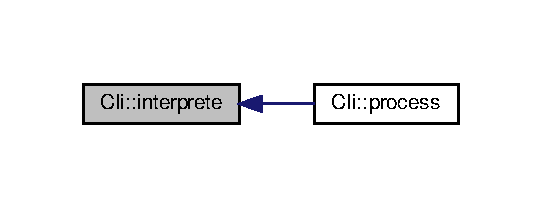
\includegraphics[width=260pt]{classCli_af29a5d8a0c3863f69c0e21133dee2d1b_icgraph}
\end{center}
\end{figure}
\mbox{\Hypertarget{classCli_a8251d6c89698aaf128318fc3ad4b2906}\label{classCli_a8251d6c89698aaf128318fc3ad4b2906}} 
\index{Cli@{Cli}!print\+Options@{print\+Options}}
\index{print\+Options@{print\+Options}!Cli@{Cli}}
\subsubsection{\texorpdfstring{print\+Options()}{printOptions()}}
{\footnotesize\ttfamily void Cli\+::print\+Options (\begin{DoxyParamCaption}{ }\end{DoxyParamCaption})\hspace{0.3cm}{\ttfamily [inline]}, {\ttfamily [private]}}



Test A private method that prints all valid options for stdin. 

\hyperlink{classCli_a8251d6c89698aaf128318fc3ad4b2906}{Cli\+::print\+Options} Here is the caller graph for this function\+:\nopagebreak
\begin{figure}[H]
\begin{center}
\leavevmode
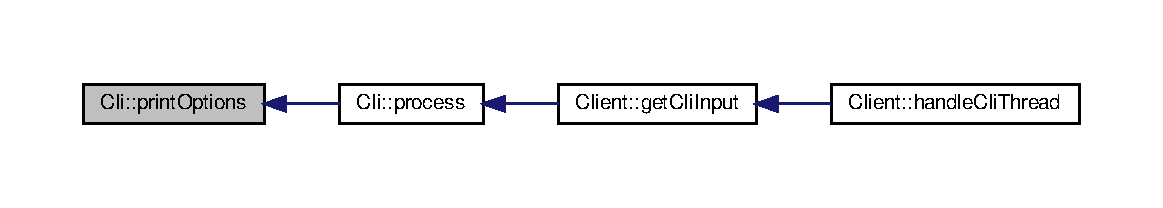
\includegraphics[width=350pt]{classCli_a8251d6c89698aaf128318fc3ad4b2906_icgraph}
\end{center}
\end{figure}
\mbox{\Hypertarget{classCli_aa2b3675ef3e3bb01ed0d1997460a0e28}\label{classCli_aa2b3675ef3e3bb01ed0d1997460a0e28}} 
\index{Cli@{Cli}!process@{process}}
\index{process@{process}!Cli@{Cli}}
\subsubsection{\texorpdfstring{process()}{process()}\hspace{0.1cm}{\footnotesize\ttfamily [1/2]}}
{\footnotesize\ttfamily \hyperlink{classRequest}{Request} Cli\+::process (\begin{DoxyParamCaption}{ }\end{DoxyParamCaption})\hspace{0.3cm}{\ttfamily [override]}, {\ttfamily [virtual]}}



Public method processing input from stdin. . 

Client\+::process() interface of \hyperlink{classCommandLineParser}{Command\+Line\+Parser} \begin{DoxyReturn}{Returns}
Vector of strings containing output from stdin. 
\end{DoxyReturn}


Implements \hyperlink{classCommandLineParser}{Command\+Line\+Parser}.

Here is the call graph for this function\+:\nopagebreak
\begin{figure}[H]
\begin{center}
\leavevmode
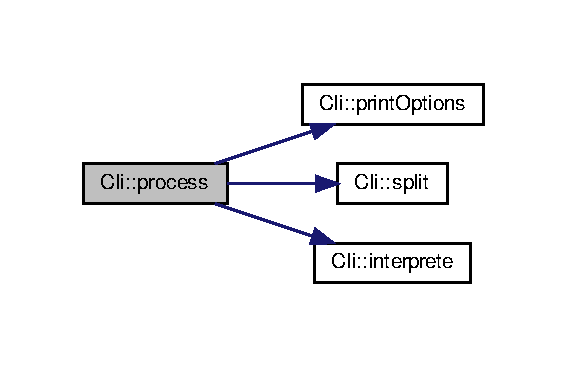
\includegraphics[width=272pt]{classCli_aa2b3675ef3e3bb01ed0d1997460a0e28_cgraph}
\end{center}
\end{figure}
Here is the caller graph for this function\+:\nopagebreak
\begin{figure}[H]
\begin{center}
\leavevmode
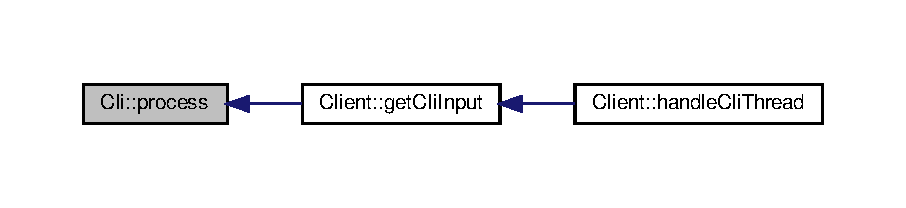
\includegraphics[width=350pt]{classCli_aa2b3675ef3e3bb01ed0d1997460a0e28_icgraph}
\end{center}
\end{figure}
\mbox{\Hypertarget{classCli_a4ee41556f8c3a736d813f0d937413da0}\label{classCli_a4ee41556f8c3a736d813f0d937413da0}} 
\index{Cli@{Cli}!process@{process}}
\index{process@{process}!Cli@{Cli}}
\subsubsection{\texorpdfstring{process()}{process()}\hspace{0.1cm}{\footnotesize\ttfamily [2/2]}}
{\footnotesize\ttfamily \hyperlink{classRequest}{Request} Cli\+::process (\begin{DoxyParamCaption}\item[{std\+::string \&}]{line }\end{DoxyParamCaption})\hspace{0.3cm}{\ttfamily [override]}, {\ttfamily [virtual]}}



Public method processing input from stdin. 

Client\+::process() interface of \hyperlink{classCommandLineParser}{Command\+Line\+Parser} 
\begin{DoxyParams}{Parameters}
{\em std\+::string\&} & fixed string used for unit testing mocking stdin \\
\hline
\end{DoxyParams}
\begin{DoxyReturn}{Returns}
Vector of strings containing output from stdin. 
\end{DoxyReturn}


Implements \hyperlink{classCommandLineParser}{Command\+Line\+Parser}.

Here is the call graph for this function\+:\nopagebreak
\begin{figure}[H]
\begin{center}
\leavevmode
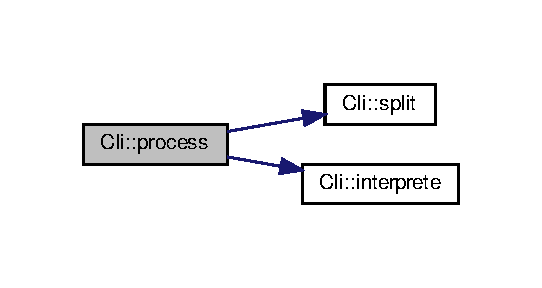
\includegraphics[width=260pt]{classCli_a4ee41556f8c3a736d813f0d937413da0_cgraph}
\end{center}
\end{figure}
\mbox{\Hypertarget{classCli_aaf60768f062a6dc2557aaddbe738a19c}\label{classCli_aaf60768f062a6dc2557aaddbe738a19c}} 
\index{Cli@{Cli}!split@{split}}
\index{split@{split}!Cli@{Cli}}
\subsubsection{\texorpdfstring{split()}{split()}}
{\footnotesize\ttfamily std\+::vector$<$std\+::string$>$ Cli\+::split (\begin{DoxyParamCaption}\item[{std\+::string \&}]{input,  }\item[{char}]{delim }\end{DoxyParamCaption})\hspace{0.3cm}{\ttfamily [inline]}, {\ttfamily [private]}}

\hyperlink{classCli_aaf60768f062a6dc2557aaddbe738a19c}{Cli\+::split}


\begin{DoxyParams}{Parameters}
{\em input} & incoming unprocessed string \\
\hline
{\em delim} & delimiter used to split \\
\hline
{\em input} & \\
\hline
\end{DoxyParams}
\begin{DoxyReturn}{Returns}

\end{DoxyReturn}

\begin{DoxyParams}{Parameters}
{\em input} & splitted into multiple strings saved in a std\+::vector \\
\hline
\end{DoxyParams}
Here is the caller graph for this function\+:\nopagebreak
\begin{figure}[H]
\begin{center}
\leavevmode
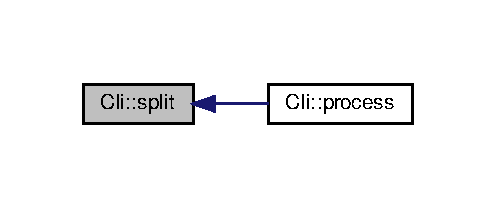
\includegraphics[width=238pt]{classCli_aaf60768f062a6dc2557aaddbe738a19c_icgraph}
\end{center}
\end{figure}


The documentation for this class was generated from the following files\+:\begin{DoxyCompactItemize}
\item 
inc/Cli.\+h\item 
src/Cli.\+cpp\end{DoxyCompactItemize}

\hypertarget{classClient}{}\section{Client Class Reference}
\label{classClient}\index{Client@{Client}}
\subsection*{Public Member Functions}
\begin{DoxyCompactItemize}
\item 
void \hyperlink{classClient_a33b0b1f7391689c68fa125549e8c5dcc}{setup} ()
\begin{DoxyCompactList}\small\item\em A method that waits C\+LI input from method get\+Cli\+Input. The method will break if input is interpreted as exit or continue by sending the request to be handled. \end{DoxyCompactList}\end{DoxyCompactItemize}
\subsection*{Public Attributes}
\begin{DoxyCompactItemize}
\item 
\mbox{\Hypertarget{classClient_a4c99f07fc4be08870e1067ba876e08fb}\label{classClient_a4c99f07fc4be08870e1067ba876e08fb}} 
Db\+Type {\bfseries type}
\end{DoxyCompactItemize}


\subsection{Member Function Documentation}
\mbox{\Hypertarget{classClient_a33b0b1f7391689c68fa125549e8c5dcc}\label{classClient_a33b0b1f7391689c68fa125549e8c5dcc}} 
\index{Client@{Client}!setup@{setup}}
\index{setup@{setup}!Client@{Client}}
\subsubsection{\texorpdfstring{setup()}{setup()}}
{\footnotesize\ttfamily void Client\+::setup (\begin{DoxyParamCaption}{ }\end{DoxyParamCaption})}



A method that waits C\+LI input from method get\+Cli\+Input. The method will break if input is interpreted as exit or continue by sending the request to be handled. 

\begin{DoxyReturn}{Returns}

\end{DoxyReturn}


The documentation for this class was generated from the following files\+:\begin{DoxyCompactItemize}
\item 
/home/mjonsson/repo/cpp\+Adv/media\+F\+W/inc/Client.\+h\item 
/home/mjonsson/repo/cpp\+Adv/media\+F\+W/src/Client.\+cpp\end{DoxyCompactItemize}

\hypertarget{classCliTest}{}\section{Cli\+Test Class Reference}
\label{classCliTest}\index{Cli\+Test@{Cli\+Test}}


Inheritance diagram for Cli\+Test\+:\nopagebreak
\begin{figure}[H]
\begin{center}
\leavevmode
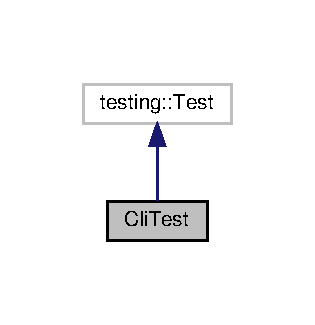
\includegraphics[width=151pt]{classCliTest__inherit__graph}
\end{center}
\end{figure}


Collaboration diagram for Cli\+Test\+:\nopagebreak
\begin{figure}[H]
\begin{center}
\leavevmode
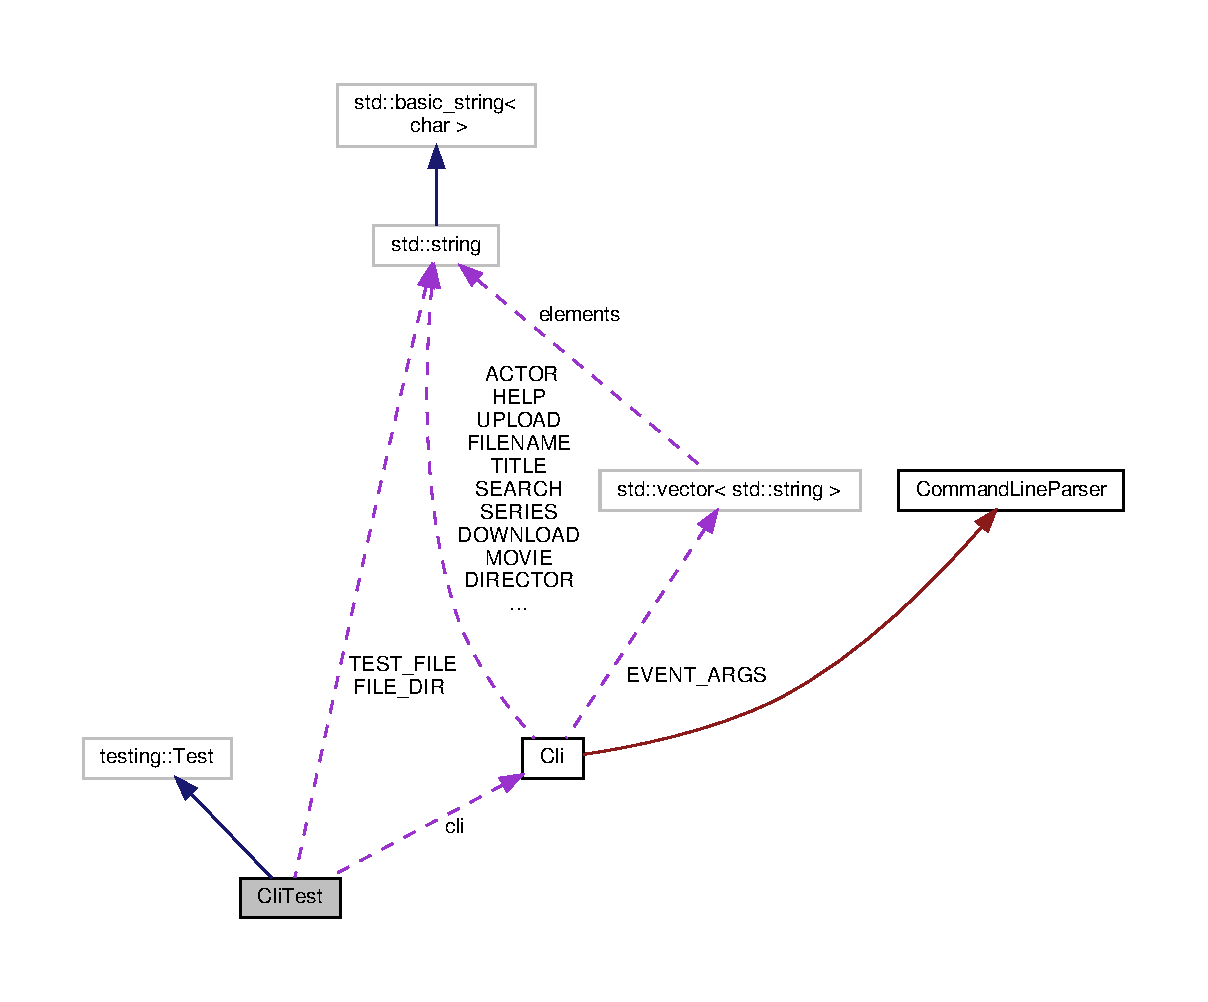
\includegraphics[width=350pt]{classCliTest__coll__graph}
\end{center}
\end{figure}
\subsection*{Protected Member Functions}
\begin{DoxyCompactItemize}
\item 
\mbox{\Hypertarget{classCliTest_a39680afdbe534fecb892079d256d7571}\label{classCliTest_a39680afdbe534fecb892079d256d7571}} 
void {\bfseries Set\+Up} ()
\item 
\mbox{\Hypertarget{classCliTest_a6a21290abec30f2e56f8b950c5a0e842}\label{classCliTest_a6a21290abec30f2e56f8b950c5a0e842}} 
void {\bfseries Tear\+Down} ()
\end{DoxyCompactItemize}
\subsection*{Protected Attributes}
\begin{DoxyCompactItemize}
\item 
\mbox{\Hypertarget{classCliTest_aa31b7626da78891c93a0c254d80acf17}\label{classCliTest_aa31b7626da78891c93a0c254d80acf17}} 
\hyperlink{classCli}{Cli} $\ast$ {\bfseries cli}
\item 
\mbox{\Hypertarget{classCliTest_a8ed91232d6341370122edb04ac2941fe}\label{classCliTest_a8ed91232d6341370122edb04ac2941fe}} 
std\+::string {\bfseries F\+I\+L\+E\+\_\+\+D\+IR} = \char`\"{}$\sim$/repo/media\+\_\+fw/media\+FW/data/\char`\"{}
\item 
\mbox{\Hypertarget{classCliTest_afa60a33336d73a6df66a0eb25329c0cc}\label{classCliTest_afa60a33336d73a6df66a0eb25329c0cc}} 
std\+::string {\bfseries T\+E\+S\+T\+\_\+\+F\+I\+LE} = F\+I\+L\+E\+\_\+\+D\+IR + \char`\"{}testfile.\+txt\char`\"{}
\item 
\mbox{\Hypertarget{classCliTest_a8a8784d4c4ca008c283eafce7ef2c470}\label{classCliTest_a8a8784d4c4ca008c283eafce7ef2c470}} 
Category {\bfseries cat2} = Category\+::\+Series
\item 
\mbox{\Hypertarget{classCliTest_a40d64f87a28cb1a15712667e17430d5a}\label{classCliTest_a40d64f87a28cb1a15712667e17430d5a}} 
Category {\bfseries cat} = Category\+::\+Movie
\end{DoxyCompactItemize}


The documentation for this class was generated from the following file\+:\begin{DoxyCompactItemize}
\item 
inc/unittests/Test\+\_\+\+Cli.\+h\end{DoxyCompactItemize}

\hypertarget{classCommandLineParser}{}\section{Command\+Line\+Parser Class Reference}
\label{classCommandLineParser}\index{Command\+Line\+Parser@{Command\+Line\+Parser}}


Inheritance diagram for Command\+Line\+Parser\+:\nopagebreak
\begin{figure}[H]
\begin{center}
\leavevmode
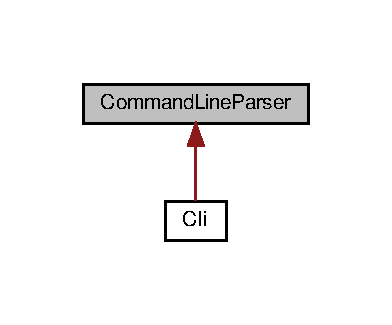
\includegraphics[width=188pt]{classCommandLineParser__inherit__graph}
\end{center}
\end{figure}
\subsection*{Public Member Functions}
\begin{DoxyCompactItemize}
\item 
\mbox{\Hypertarget{classCommandLineParser_a40f670282d5f52b4a2bcf61701e016e3}\label{classCommandLineParser_a40f670282d5f52b4a2bcf61701e016e3}} 
virtual \hyperlink{classRequest}{Request} {\bfseries process} ()=0
\item 
\mbox{\Hypertarget{classCommandLineParser_a0449154ff3be82b1ee2c125af2874f49}\label{classCommandLineParser_a0449154ff3be82b1ee2c125af2874f49}} 
virtual \hyperlink{classRequest}{Request} {\bfseries process} (std\+::string \&)=0
\item 
\mbox{\Hypertarget{classCommandLineParser_a7ed2465a960c5cee78d324922214ec1c}\label{classCommandLineParser_a7ed2465a960c5cee78d324922214ec1c}} 
virtual \hyperlink{classRequest}{Request} {\bfseries interprete} (std\+::vector$<$ std\+::string $>$ \&)=0
\end{DoxyCompactItemize}


The documentation for this class was generated from the following file\+:\begin{DoxyCompactItemize}
\item 
inc/ifc/Command\+Line\+Parser.\+h\end{DoxyCompactItemize}

\hypertarget{classConnection}{}\section{Connection Class Reference}
\label{classConnection}\index{Connection@{Connection}}
\subsection*{Public Member Functions}
\begin{DoxyCompactItemize}
\item 
\mbox{\Hypertarget{classConnection_a4cbf33699e3ca42a23eb8168be4d5287}\label{classConnection_a4cbf33699e3ca42a23eb8168be4d5287}} 
bool {\bfseries get\+Connection\+Status} ()
\item 
\mbox{\Hypertarget{classConnection_ab59a9e6d364eff3f116e60b6ccc60f1b}\label{classConnection_ab59a9e6d364eff3f116e60b6ccc60f1b}} 
bool {\bfseries send\+Remote\+Commands} (std\+::string request, std\+::string \&result)
\end{DoxyCompactItemize}


The documentation for this class was generated from the following files\+:\begin{DoxyCompactItemize}
\item 
/home/mjonsson/repo/cpp\+Adv/media\+F\+W/inc/Connection.\+h\item 
/home/mjonsson/repo/cpp\+Adv/media\+F\+W/src/Connection.\+cpp\end{DoxyCompactItemize}

\hypertarget{classConnectionStream}{}\section{Connection\+Stream Class Reference}
\label{classConnectionStream}\index{Connection\+Stream@{Connection\+Stream}}


Collaboration diagram for Connection\+Stream\+:\nopagebreak
\begin{figure}[H]
\begin{center}
\leavevmode
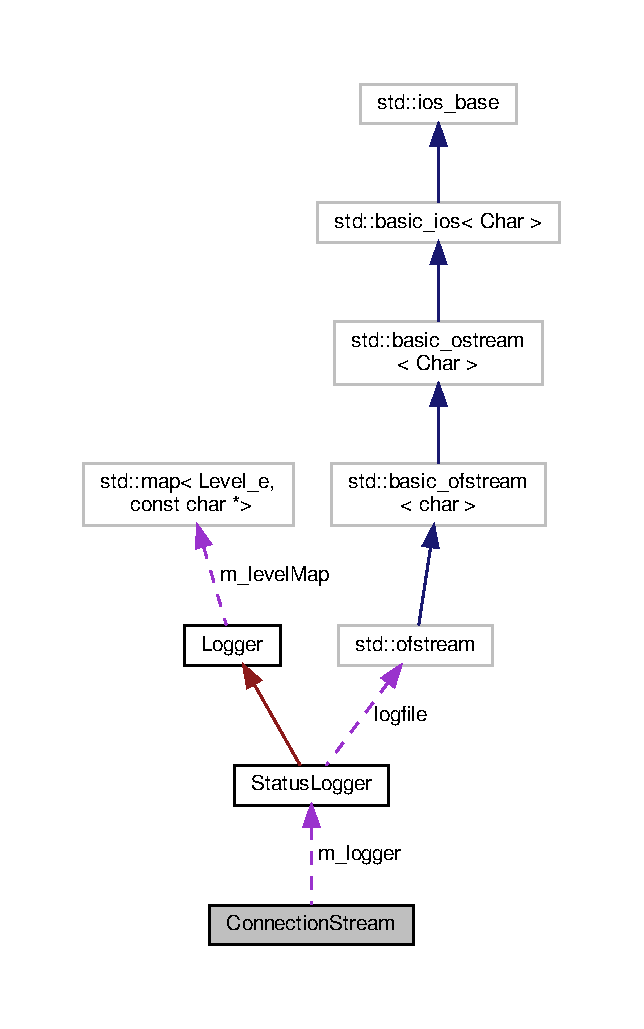
\includegraphics[width=309pt]{classConnectionStream__coll__graph}
\end{center}
\end{figure}
\subsection*{Public Member Functions}
\begin{DoxyCompactItemize}
\item 
\mbox{\Hypertarget{classConnectionStream_a90b1fa3e20b531f40b5dff907ebe6e75}\label{classConnectionStream_a90b1fa3e20b531f40b5dff907ebe6e75}} 
{\bfseries Connection\+Stream} (ssh\+\_\+session session)
\item 
\mbox{\Hypertarget{classConnectionStream_a3e15cc23cc086eab18ac6ca4a084fe72}\label{classConnectionStream_a3e15cc23cc086eab18ac6ca4a084fe72}} 
bool {\bfseries send\+Remote\+Commands} (std\+::string \&request, std\+::string \&result)
\end{DoxyCompactItemize}
\subsection*{Private Member Functions}
\begin{DoxyCompactItemize}
\item 
\mbox{\Hypertarget{classConnectionStream_a42f6169f1228c0f690d385fc5a278965}\label{classConnectionStream_a42f6169f1228c0f690d385fc5a278965}} 
void {\bfseries close\+Channel} (ssh\+\_\+channel channel)
\end{DoxyCompactItemize}
\subsection*{Private Attributes}
\begin{DoxyCompactItemize}
\item 
\mbox{\Hypertarget{classConnectionStream_a0c3d09410dad1e406954bb61fd9d64b9}\label{classConnectionStream_a0c3d09410dad1e406954bb61fd9d64b9}} 
ssh\+\_\+session {\bfseries m\+\_\+session}
\item 
\mbox{\Hypertarget{classConnectionStream_a63c356309a1cfa4ac04f7dc5b2c08fa0}\label{classConnectionStream_a63c356309a1cfa4ac04f7dc5b2c08fa0}} 
ssh\+\_\+channel {\bfseries m\+\_\+channel}
\item 
\mbox{\Hypertarget{classConnectionStream_a34222df0c29e871cf31b44c53fdc017a}\label{classConnectionStream_a34222df0c29e871cf31b44c53fdc017a}} 
\hyperlink{classStatusLogger}{Status\+Logger} $\ast$ {\bfseries m\+\_\+logger}
\end{DoxyCompactItemize}


The documentation for this class was generated from the following file\+:\begin{DoxyCompactItemize}
\item 
inc/Connection\+Stream.\+h\end{DoxyCompactItemize}

\hypertarget{classConnector}{}\section{Connector Class Reference}
\label{classConnector}\index{Connector@{Connector}}


Inheritance diagram for Connector\+:\nopagebreak
\begin{figure}[H]
\begin{center}
\leavevmode
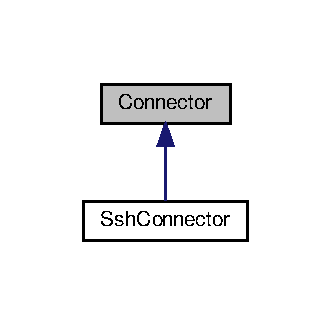
\includegraphics[width=159pt]{classConnector__inherit__graph}
\end{center}
\end{figure}
\subsection*{Public Member Functions}
\begin{DoxyCompactItemize}
\item 
\mbox{\Hypertarget{classConnector_a54e1432219a30649a9eb2bfd7e9ff89e}\label{classConnector_a54e1432219a30649a9eb2bfd7e9ff89e}} 
virtual \hyperlink{classConnectionStream}{Connection\+Stream} $\ast$ {\bfseries connect} (uint16\+\_\+t port, std\+::string server)=0
\item 
\mbox{\Hypertarget{classConnector_afec79f2f375e2e1bca502602aed6b129}\label{classConnector_afec79f2f375e2e1bca502602aed6b129}} 
virtual void {\bfseries disconnect} ()=0
\end{DoxyCompactItemize}
\subsection*{Protected Member Functions}
\begin{DoxyCompactItemize}
\item 
\mbox{\Hypertarget{classConnector_a4e63ecab513194724dc6a4e84068bcb5}\label{classConnector_a4e63ecab513194724dc6a4e84068bcb5}} 
virtual int {\bfseries resolve\+Host} (ssh\+\_\+session session)=0
\end{DoxyCompactItemize}


The documentation for this class was generated from the following file\+:\begin{DoxyCompactItemize}
\item 
inc/ifc/Connector.\+h\end{DoxyCompactItemize}

\hypertarget{classDatabase}{}\section{Database Class Reference}
\label{classDatabase}\index{Database@{Database}}


Defines methods for database implementations.  




Inheritance diagram for Database\+:\nopagebreak
\begin{figure}[H]
\begin{center}
\leavevmode
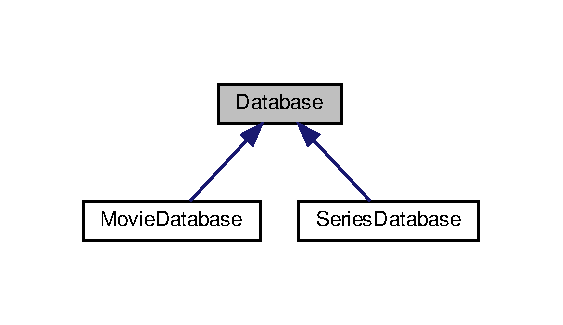
\includegraphics[width=270pt]{classDatabase__inherit__graph}
\end{center}
\end{figure}


Collaboration diagram for Database\+:\nopagebreak
\begin{figure}[H]
\begin{center}
\leavevmode
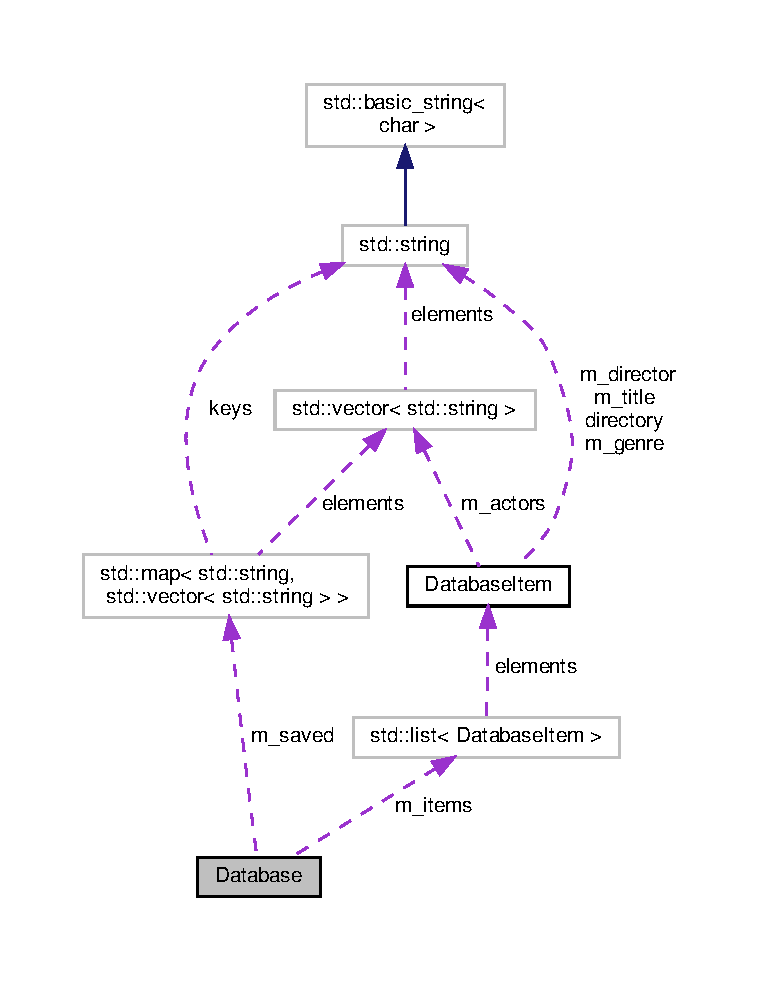
\includegraphics[width=350pt]{classDatabase__coll__graph}
\end{center}
\end{figure}
\subsection*{Public Member Functions}
\begin{DoxyCompactItemize}
\item 
\hyperlink{classDatabase_aa57fbada3001c2db58a0ca6c7071bd18}{Database} ()=default
\begin{DoxyCompactList}\small\item\em Default constructor. \end{DoxyCompactList}\item 
\hyperlink{classDatabase_a341cd0fe8c615e829e3a22b74c208bb5}{$\sim$\+Database} ()=default
\begin{DoxyCompactList}\small\item\em Default deconstructor. \end{DoxyCompactList}\item 
virtual void \hyperlink{classDatabase_a14d24487b4ea3b50097b9ac0f2b3f317}{sync\+Local\+Database} ()
\begin{DoxyCompactList}\small\item\em Sync info from json file and saves it to a list of database objects. \end{DoxyCompactList}\item 
virtual void \hyperlink{classDatabase_a80fa14ab9f4deadc9a2ab7493f1919a4}{push\+Item} (const \hyperlink{classDatabaseItem}{Database\+Item} \&m\+\_\+item)
\begin{DoxyCompactList}\small\item\em Uploads the requested database item. \end{DoxyCompactList}\item 
virtual \hyperlink{classDatabaseItem}{Database\+Item} \hyperlink{classDatabase_a40254eec69c7d7cc15da24a9f0b072b3}{fetch\+Item} (const std\+::string \&title)
\begin{DoxyCompactList}\small\item\em Fetch the requested database item. \end{DoxyCompactList}\item 
virtual void \hyperlink{classDatabase_a8f47437526eeec631f1328fab9bbbc75}{purge\+Item} (\hyperlink{classDatabaseItem}{Database\+Item} m\+\_\+item)
\begin{DoxyCompactList}\small\item\em Delete the requested database item. \end{DoxyCompactList}\item 
virtual void \hyperlink{classDatabase_afa345da530fd5c8dfe0c978917cd6049}{print\+All} ()
\begin{DoxyCompactList}\small\item\em Prints the entire database content. \end{DoxyCompactList}\item 
virtual long \hyperlink{classDatabase_a230225cb341eb23a99a83ef3d1abae53}{get\+Number\+Of\+Item} ()
\begin{DoxyCompactList}\small\item\em Method that return the size of the database. \end{DoxyCompactList}\end{DoxyCompactItemize}
\subsection*{Protected Attributes}
\begin{DoxyCompactItemize}
\item 
std\+::list$<$ \hyperlink{classDatabaseItem}{Database\+Item} $>$ \hyperlink{classDatabase_a5a4ac1f3bf0f5fd77a696174ad9e5c45}{m\+\_\+items}
\begin{DoxyCompactList}\small\item\em A protected list of Database\+Items. \end{DoxyCompactList}\item 
std\+::map$<$ std\+::string, std\+::vector$<$ std\+::string $>$ $>$ \hyperlink{classDatabase_a9f87cbe5a1be71d541083dffa8d8c9ad}{m\+\_\+saved}
\begin{DoxyCompactList}\small\item\em A protected vector of strings with info for the Database\+Items. \end{DoxyCompactList}\item 
std\+::mutex \hyperlink{classDatabase_a7f55f3a5d93c9694ee4f08a2f2135b1d}{m\+\_\+lock}
\begin{DoxyCompactList}\small\item\em A protected mutex for threadsafe r/w of Database\+Items. \end{DoxyCompactList}\item 
std\+::condition\+\_\+variable \hyperlink{classDatabase_a2ad8bf38964b3e18a0e168437acbdb27}{m\+\_\+empty\+List}
\begin{DoxyCompactList}\small\item\em A protected condittion variable for the mutex and \hyperlink{classDatabase}{Database} list. \end{DoxyCompactList}\end{DoxyCompactItemize}


\subsection{Detailed Description}
Defines methods for database implementations. 



\subsection{Constructor \& Destructor Documentation}
\mbox{\Hypertarget{classDatabase_aa57fbada3001c2db58a0ca6c7071bd18}\label{classDatabase_aa57fbada3001c2db58a0ca6c7071bd18}} 
\index{Database@{Database}!Database@{Database}}
\index{Database@{Database}!Database@{Database}}
\subsubsection{\texorpdfstring{Database()}{Database()}}
{\footnotesize\ttfamily Database\+::\+Database (\begin{DoxyParamCaption}{ }\end{DoxyParamCaption})\hspace{0.3cm}{\ttfamily [default]}}



Default constructor. 

\hyperlink{classDatabase_aa57fbada3001c2db58a0ca6c7071bd18}{Database()} \mbox{\Hypertarget{classDatabase_a341cd0fe8c615e829e3a22b74c208bb5}\label{classDatabase_a341cd0fe8c615e829e3a22b74c208bb5}} 
\index{Database@{Database}!````~Database@{$\sim$\+Database}}
\index{````~Database@{$\sim$\+Database}!Database@{Database}}
\subsubsection{\texorpdfstring{$\sim$\+Database()}{~Database()}}
{\footnotesize\ttfamily Database\+::$\sim$\+Database (\begin{DoxyParamCaption}{ }\end{DoxyParamCaption})\hspace{0.3cm}{\ttfamily [default]}}



Default deconstructor. 

\hyperlink{classDatabase_a341cd0fe8c615e829e3a22b74c208bb5}{$\sim$\+Database()} 

\subsection{Member Function Documentation}
\mbox{\Hypertarget{classDatabase_a40254eec69c7d7cc15da24a9f0b072b3}\label{classDatabase_a40254eec69c7d7cc15da24a9f0b072b3}} 
\index{Database@{Database}!fetch\+Item@{fetch\+Item}}
\index{fetch\+Item@{fetch\+Item}!Database@{Database}}
\subsubsection{\texorpdfstring{fetch\+Item()}{fetchItem()}}
{\footnotesize\ttfamily virtual \hyperlink{classDatabaseItem}{Database\+Item} Database\+::fetch\+Item (\begin{DoxyParamCaption}\item[{const std\+::string \&}]{title }\end{DoxyParamCaption})\hspace{0.3cm}{\ttfamily [inline]}, {\ttfamily [virtual]}}



Fetch the requested database item. 

A const reference to a title

\begin{DoxyReturn}{Returns}
The requested \hyperlink{classDatabaseItem}{Database\+Item}
\end{DoxyReturn}


Reimplemented in \hyperlink{classMovieDatabase_ac0bb39b8be599ffea76081809ae42dda}{Movie\+Database}, and \hyperlink{classSeriesDatabase_af5303a723910395b31f2e01088de9130}{Series\+Database}.

\mbox{\Hypertarget{classDatabase_a230225cb341eb23a99a83ef3d1abae53}\label{classDatabase_a230225cb341eb23a99a83ef3d1abae53}} 
\index{Database@{Database}!get\+Number\+Of\+Item@{get\+Number\+Of\+Item}}
\index{get\+Number\+Of\+Item@{get\+Number\+Of\+Item}!Database@{Database}}
\subsubsection{\texorpdfstring{get\+Number\+Of\+Item()}{getNumberOfItem()}}
{\footnotesize\ttfamily virtual long Database\+::get\+Number\+Of\+Item (\begin{DoxyParamCaption}{ }\end{DoxyParamCaption})\hspace{0.3cm}{\ttfamily [inline]}, {\ttfamily [virtual]}}



Method that return the size of the database. 

\begin{DoxyReturn}{Returns}
Size of the database (long).
\end{DoxyReturn}


Reimplemented in \hyperlink{classMovieDatabase_a9a386f51dd72d63414a124cbcfcd879b}{Movie\+Database}, and \hyperlink{classSeriesDatabase_af5fe5a423303eff4489a7679907ef994}{Series\+Database}.

\mbox{\Hypertarget{classDatabase_afa345da530fd5c8dfe0c978917cd6049}\label{classDatabase_afa345da530fd5c8dfe0c978917cd6049}} 
\index{Database@{Database}!print\+All@{print\+All}}
\index{print\+All@{print\+All}!Database@{Database}}
\subsubsection{\texorpdfstring{print\+All()}{printAll()}}
{\footnotesize\ttfamily virtual void Database\+::print\+All (\begin{DoxyParamCaption}{ }\end{DoxyParamCaption})\hspace{0.3cm}{\ttfamily [inline]}, {\ttfamily [virtual]}}



Prints the entire database content. 

s 

Reimplemented in \hyperlink{classMovieDatabase_af1e13b6fc0fd7186e98edbe2cf187618}{Movie\+Database}, and \hyperlink{classSeriesDatabase_ae2bf5323216e0043292494d3f0ac978c}{Series\+Database}.

\mbox{\Hypertarget{classDatabase_a8f47437526eeec631f1328fab9bbbc75}\label{classDatabase_a8f47437526eeec631f1328fab9bbbc75}} 
\index{Database@{Database}!purge\+Item@{purge\+Item}}
\index{purge\+Item@{purge\+Item}!Database@{Database}}
\subsubsection{\texorpdfstring{purge\+Item()}{purgeItem()}}
{\footnotesize\ttfamily virtual void Database\+::purge\+Item (\begin{DoxyParamCaption}\item[{\hyperlink{classDatabaseItem}{Database\+Item}}]{m\+\_\+item }\end{DoxyParamCaption})\hspace{0.3cm}{\ttfamily [inline]}, {\ttfamily [virtual]}}



Delete the requested database item. 

A const reference to a database item

Reimplemented in \hyperlink{classMovieDatabase_ad3ce59d0fa7f64937085e7504bd3b85a}{Movie\+Database}, and \hyperlink{classSeriesDatabase_a863a35987b5a4de15a121b8b4358e353}{Series\+Database}.

\mbox{\Hypertarget{classDatabase_a80fa14ab9f4deadc9a2ab7493f1919a4}\label{classDatabase_a80fa14ab9f4deadc9a2ab7493f1919a4}} 
\index{Database@{Database}!push\+Item@{push\+Item}}
\index{push\+Item@{push\+Item}!Database@{Database}}
\subsubsection{\texorpdfstring{push\+Item()}{pushItem()}}
{\footnotesize\ttfamily virtual void Database\+::push\+Item (\begin{DoxyParamCaption}\item[{const \hyperlink{classDatabaseItem}{Database\+Item} \&}]{m\+\_\+item }\end{DoxyParamCaption})\hspace{0.3cm}{\ttfamily [inline]}, {\ttfamily [virtual]}}



Uploads the requested database item. 

A const reference to a database item

Reimplemented in \hyperlink{classMovieDatabase_a203b9b5c1b325997ce519859a436b6ce}{Movie\+Database}, and \hyperlink{classSeriesDatabase_a7591f89ab256d9f5a41235f5552e4e23}{Series\+Database}.

\mbox{\Hypertarget{classDatabase_a14d24487b4ea3b50097b9ac0f2b3f317}\label{classDatabase_a14d24487b4ea3b50097b9ac0f2b3f317}} 
\index{Database@{Database}!sync\+Local\+Database@{sync\+Local\+Database}}
\index{sync\+Local\+Database@{sync\+Local\+Database}!Database@{Database}}
\subsubsection{\texorpdfstring{sync\+Local\+Database()}{syncLocalDatabase()}}
{\footnotesize\ttfamily virtual void Database\+::sync\+Local\+Database (\begin{DoxyParamCaption}{ }\end{DoxyParamCaption})\hspace{0.3cm}{\ttfamily [inline]}, {\ttfamily [virtual]}}



Sync info from json file and saves it to a list of database objects. 

Database\+::sync\+Database() 

Reimplemented in \hyperlink{classMovieDatabase_aee175db6a2a357b6180fcab5d57eddd5}{Movie\+Database}, and \hyperlink{classSeriesDatabase_a0ba159b6d52a3cfa07135c7d8b37ef76}{Series\+Database}.



\subsection{Member Data Documentation}
\mbox{\Hypertarget{classDatabase_a2ad8bf38964b3e18a0e168437acbdb27}\label{classDatabase_a2ad8bf38964b3e18a0e168437acbdb27}} 
\index{Database@{Database}!m\+\_\+empty\+List@{m\+\_\+empty\+List}}
\index{m\+\_\+empty\+List@{m\+\_\+empty\+List}!Database@{Database}}
\subsubsection{\texorpdfstring{m\+\_\+empty\+List}{m\_emptyList}}
{\footnotesize\ttfamily std\+::condition\+\_\+variable Database\+::m\+\_\+empty\+List\hspace{0.3cm}{\ttfamily [protected]}}



A protected condittion variable for the mutex and \hyperlink{classDatabase}{Database} list. 

\mbox{\Hypertarget{classDatabase_a5a4ac1f3bf0f5fd77a696174ad9e5c45}\label{classDatabase_a5a4ac1f3bf0f5fd77a696174ad9e5c45}} 
\index{Database@{Database}!m\+\_\+items@{m\+\_\+items}}
\index{m\+\_\+items@{m\+\_\+items}!Database@{Database}}
\subsubsection{\texorpdfstring{m\+\_\+items}{m\_items}}
{\footnotesize\ttfamily std\+::list$<$\hyperlink{classDatabaseItem}{Database\+Item}$>$ Database\+::m\+\_\+items\hspace{0.3cm}{\ttfamily [protected]}}



A protected list of Database\+Items. 

\mbox{\Hypertarget{classDatabase_a7f55f3a5d93c9694ee4f08a2f2135b1d}\label{classDatabase_a7f55f3a5d93c9694ee4f08a2f2135b1d}} 
\index{Database@{Database}!m\+\_\+lock@{m\+\_\+lock}}
\index{m\+\_\+lock@{m\+\_\+lock}!Database@{Database}}
\subsubsection{\texorpdfstring{m\+\_\+lock}{m\_lock}}
{\footnotesize\ttfamily std\+::mutex Database\+::m\+\_\+lock\hspace{0.3cm}{\ttfamily [mutable]}, {\ttfamily [protected]}}



A protected mutex for threadsafe r/w of Database\+Items. 

\mbox{\Hypertarget{classDatabase_a9f87cbe5a1be71d541083dffa8d8c9ad}\label{classDatabase_a9f87cbe5a1be71d541083dffa8d8c9ad}} 
\index{Database@{Database}!m\+\_\+saved@{m\+\_\+saved}}
\index{m\+\_\+saved@{m\+\_\+saved}!Database@{Database}}
\subsubsection{\texorpdfstring{m\+\_\+saved}{m\_saved}}
{\footnotesize\ttfamily std\+::map$<$std\+::string, std\+::vector$<$std\+::string$>$ $>$ Database\+::m\+\_\+saved\hspace{0.3cm}{\ttfamily [protected]}}



A protected vector of strings with info for the Database\+Items. 



The documentation for this class was generated from the following file\+:\begin{DoxyCompactItemize}
\item 
inc/database/Database.\+h\end{DoxyCompactItemize}

\hypertarget{classDatabaseItem}{}\section{Database\+Item Class Reference}
\label{classDatabaseItem}\index{Database\+Item@{Database\+Item}}


Collaboration diagram for Database\+Item\+:
\nopagebreak
\begin{figure}[H]
\begin{center}
\leavevmode
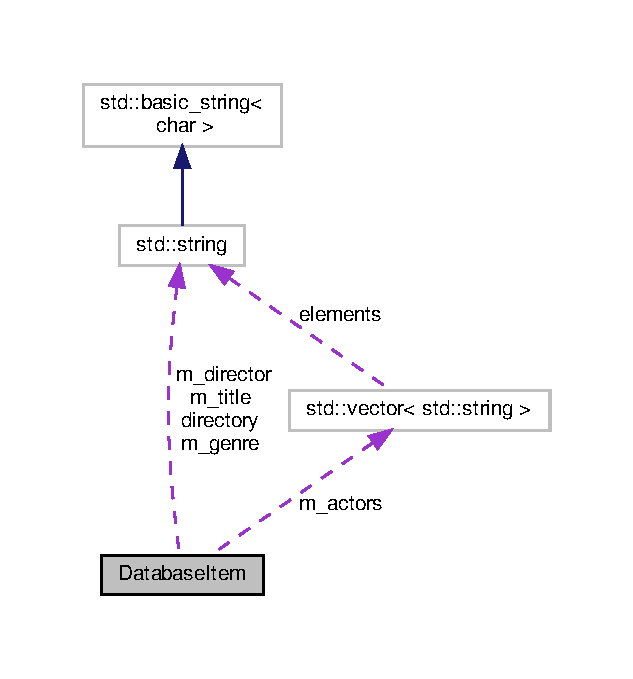
\includegraphics[width=330pt]{classDatabaseItem__coll__graph}
\end{center}
\end{figure}
\subsection*{Public Member Functions}
\begin{DoxyCompactItemize}
\item 
\mbox{\Hypertarget{classDatabaseItem_abb8e57f5ec53e855c541e5b27c4dfe10}\label{classDatabaseItem_abb8e57f5ec53e855c541e5b27c4dfe10}} 
{\bfseries Database\+Item} (std\+::vector$<$ std\+::string $>$ \+\_\+actors, std\+::string \+\_\+title, std\+::string \+\_\+genre, std\+::string \+\_\+director)
\item 
\mbox{\Hypertarget{classDatabaseItem_a51f4dbeb282806b7ac10e6b49b90eeef}\label{classDatabaseItem_a51f4dbeb282806b7ac10e6b49b90eeef}} 
void {\bfseries set\+Feature} (\hyperlink{structTags}{Tags} feature)
\item 
\mbox{\Hypertarget{classDatabaseItem_a98560961c4ab1266fe9b10f094bea568}\label{classDatabaseItem_a98560961c4ab1266fe9b10f094bea568}} 
std\+::vector$<$ std\+::string $>$ {\bfseries get\+Actors} ()
\item 
\mbox{\Hypertarget{classDatabaseItem_a87f2ebf677aaec4bc2e95eea2b7bd329}\label{classDatabaseItem_a87f2ebf677aaec4bc2e95eea2b7bd329}} 
std\+::string {\bfseries get\+Title} () const
\item 
\mbox{\Hypertarget{classDatabaseItem_a7edc61bf54ac2e48e921b9948d9efecb}\label{classDatabaseItem_a7edc61bf54ac2e48e921b9948d9efecb}} 
std\+::string {\bfseries get\+Director} ()
\item 
\mbox{\Hypertarget{classDatabaseItem_ac1d9f64c889ed271aa0f586a62a2c82a}\label{classDatabaseItem_ac1d9f64c889ed271aa0f586a62a2c82a}} 
std\+::string {\bfseries get\+Genre} ()
\item 
\mbox{\Hypertarget{classDatabaseItem_afcca0a554ac65bdcf796480e8d2920f4}\label{classDatabaseItem_afcca0a554ac65bdcf796480e8d2920f4}} 
std\+::string {\bfseries get\+Dir} ()
\end{DoxyCompactItemize}
\subsection*{Private Attributes}
\begin{DoxyCompactItemize}
\item 
\mbox{\Hypertarget{classDatabaseItem_a5ecbf8e196e110a738bb8ab1fbdff80b}\label{classDatabaseItem_a5ecbf8e196e110a738bb8ab1fbdff80b}} 
std\+::string {\bfseries directory}
\item 
\mbox{\Hypertarget{classDatabaseItem_aae3a4413ab461a85af2e79c0491a4e51}\label{classDatabaseItem_aae3a4413ab461a85af2e79c0491a4e51}} 
std\+::string {\bfseries m\+\_\+title}
\item 
\mbox{\Hypertarget{classDatabaseItem_a31482f012b886663cd8f2374e5bfe715}\label{classDatabaseItem_a31482f012b886663cd8f2374e5bfe715}} 
std\+::string {\bfseries m\+\_\+genre}
\item 
\mbox{\Hypertarget{classDatabaseItem_ad83b8f7fe4c6de1a3440ee3397192b01}\label{classDatabaseItem_ad83b8f7fe4c6de1a3440ee3397192b01}} 
std\+::string {\bfseries m\+\_\+director}
\item 
\mbox{\Hypertarget{classDatabaseItem_af98cce4f0865b2bf17d6a484c17ffaf9}\label{classDatabaseItem_af98cce4f0865b2bf17d6a484c17ffaf9}} 
std\+::vector$<$ std\+::string $>$ {\bfseries m\+\_\+actors}
\end{DoxyCompactItemize}


The documentation for this class was generated from the following file\+:\begin{DoxyCompactItemize}
\item 
/home/mjonsson/repo/cpp\+Adv/media\+F\+W/inc/\+Database/Database\+Item.\+h\end{DoxyCompactItemize}

\hypertarget{classJsonParser}{}\section{Json\+Parser Class Reference}
\label{classJsonParser}\index{Json\+Parser@{Json\+Parser}}


Inheritance diagram for Json\+Parser\+:\nopagebreak
\begin{figure}[H]
\begin{center}
\leavevmode
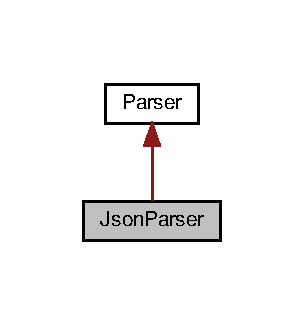
\includegraphics[width=146pt]{classJsonParser__inherit__graph}
\end{center}
\end{figure}


Collaboration diagram for Json\+Parser\+:\nopagebreak
\begin{figure}[H]
\begin{center}
\leavevmode
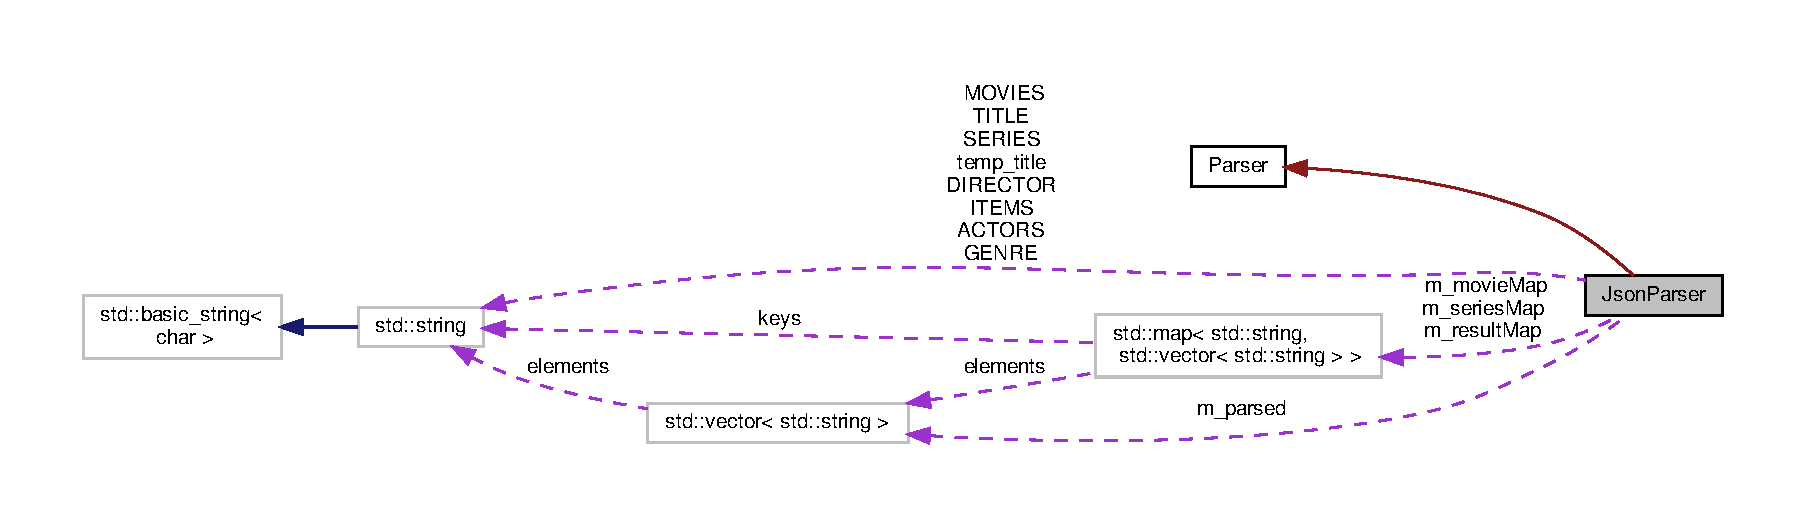
\includegraphics[width=350pt]{classJsonParser__coll__graph}
\end{center}
\end{figure}
\subsection*{Public Member Functions}
\begin{DoxyCompactItemize}
\item 
\mbox{\Hypertarget{classJsonParser_af6b90af892f999ee37dfc57bc0a7851f}\label{classJsonParser_af6b90af892f999ee37dfc57bc0a7851f}} 
{\bfseries Json\+Parser} (\hyperlink{classJsonParser}{Json\+Parser} const \&)=delete
\item 
\mbox{\Hypertarget{classJsonParser_ab4f43720d31047a61275598769b30e7d}\label{classJsonParser_ab4f43720d31047a61275598769b30e7d}} 
void {\bfseries operator=} (\hyperlink{classJsonParser}{Json\+Parser} const \&)=delete
\item 
\mbox{\Hypertarget{classJsonParser_a1d091b22b4f95ea1c16e9d09b644715e}\label{classJsonParser_a1d091b22b4f95ea1c16e9d09b644715e}} 
void {\bfseries clear} () override
\item 
\mbox{\Hypertarget{classJsonParser_abd179a463a5ce61bad930af35bf414d8}\label{classJsonParser_abd179a463a5ce61bad930af35bf414d8}} 
void {\bfseries load} (const Category \&) override
\item 
\mbox{\Hypertarget{classJsonParser_a9ab6146344e60e607289dafe2609c4e5}\label{classJsonParser_a9ab6146344e60e607289dafe2609c4e5}} 
void {\bfseries add} (const Category \&, \hyperlink{classDatabaseItem}{Database\+Item} \&) override
\item 
\mbox{\Hypertarget{classJsonParser_ad49a8004db93e654df391bac2d98c5cc}\label{classJsonParser_ad49a8004db93e654df391bac2d98c5cc}} 
void {\bfseries remove} (const Category \&, \hyperlink{classDatabaseItem}{Database\+Item} \&) override
\item 
\mbox{\Hypertarget{classJsonParser_af5641c4ab20251540d9c9f7a8d182efb}\label{classJsonParser_af5641c4ab20251540d9c9f7a8d182efb}} 
bool {\bfseries find} (Category \&, const std\+::string \&) override
\item 
\mbox{\Hypertarget{classJsonParser_a06078f0464569dac47c5d66131a4f8a4}\label{classJsonParser_a06078f0464569dac47c5d66131a4f8a4}} 
std\+::map$<$ std\+::string, std\+::vector$<$ std\+::string $>$ $>$ {\bfseries get\+Movie\+Parsed} ()
\item 
\mbox{\Hypertarget{classJsonParser_ac942ea55db61a23fd1c6106b76ad1fa4}\label{classJsonParser_ac942ea55db61a23fd1c6106b76ad1fa4}} 
std\+::map$<$ std\+::string, std\+::vector$<$ std\+::string $>$ $>$ {\bfseries get\+Series\+Parsed} ()
\item 
\mbox{\Hypertarget{classJsonParser_ab23dd51f8c905cc86d2ad0b9bf232aeb}\label{classJsonParser_ab23dd51f8c905cc86d2ad0b9bf232aeb}} 
std\+::map$<$ std\+::string, std\+::vector$<$ std\+::string $>$ $>$ {\bfseries get\+Latest\+Result} ()
\end{DoxyCompactItemize}
\subsection*{Static Public Member Functions}
\begin{DoxyCompactItemize}
\item 
\mbox{\Hypertarget{classJsonParser_a31933a8a827a8377b5edbf01bd4a66ac}\label{classJsonParser_a31933a8a827a8377b5edbf01bd4a66ac}} 
static \hyperlink{classJsonParser}{Json\+Parser} \& {\bfseries get\+Instance} ()
\end{DoxyCompactItemize}
\subsection*{Private Attributes}
\begin{DoxyCompactItemize}
\item 
\mbox{\Hypertarget{classJsonParser_a1fd58d33ddee29187d335f9f0cf0a0db}\label{classJsonParser_a1fd58d33ddee29187d335f9f0cf0a0db}} 
const std\+::string {\bfseries T\+I\+T\+LE} = \char`\"{}title\char`\"{}
\item 
\mbox{\Hypertarget{classJsonParser_a32223885ef9b529e156fb47ea847abff}\label{classJsonParser_a32223885ef9b529e156fb47ea847abff}} 
const std\+::string {\bfseries G\+E\+N\+RE} = \char`\"{}genre\char`\"{}
\item 
\mbox{\Hypertarget{classJsonParser_ad47cedc2b9fc664735a9fdcbc9869033}\label{classJsonParser_ad47cedc2b9fc664735a9fdcbc9869033}} 
const std\+::string {\bfseries A\+C\+T\+O\+RS} = \char`\"{}actors\char`\"{}
\item 
\mbox{\Hypertarget{classJsonParser_a8d6aa8c21e729236fd180f051358e9c9}\label{classJsonParser_a8d6aa8c21e729236fd180f051358e9c9}} 
const std\+::string {\bfseries D\+I\+R\+E\+C\+T\+OR} = \char`\"{}director\char`\"{}
\item 
\mbox{\Hypertarget{classJsonParser_a3fcbbf58d72ac41ef6caf67cb34b7864}\label{classJsonParser_a3fcbbf58d72ac41ef6caf67cb34b7864}} 
const std\+::string {\bfseries I\+T\+E\+MS} = \char`\"{}items\char`\"{}
\item 
\mbox{\Hypertarget{classJsonParser_ab209a873c5fa7850d80e9ddc9bab04c0}\label{classJsonParser_ab209a873c5fa7850d80e9ddc9bab04c0}} 
std\+::string {\bfseries M\+O\+V\+I\+ES} = \char`\"{}Movies\char`\"{}
\item 
\mbox{\Hypertarget{classJsonParser_a00fe1d9101a48ef93ee8eeabcc059aae}\label{classJsonParser_a00fe1d9101a48ef93ee8eeabcc059aae}} 
std\+::string {\bfseries S\+E\+R\+I\+ES} = \char`\"{}Series\char`\"{}
\item 
\mbox{\Hypertarget{classJsonParser_ae5a993adef29a11237804dfd3de9fd50}\label{classJsonParser_ae5a993adef29a11237804dfd3de9fd50}} 
Json\+::\+Value {\bfseries m\+\_\+root}
\item 
\mbox{\Hypertarget{classJsonParser_a1947ab7e13cc7917154d7d8aea23f777}\label{classJsonParser_a1947ab7e13cc7917154d7d8aea23f777}} 
std\+::string {\bfseries temp\+\_\+title}
\item 
\mbox{\Hypertarget{classJsonParser_a33e76488d7685330236a52de4a186aba}\label{classJsonParser_a33e76488d7685330236a52de4a186aba}} 
std\+::vector$<$ std\+::string $>$ {\bfseries m\+\_\+parsed}
\item 
\mbox{\Hypertarget{classJsonParser_ad89def06854ea0cf7d21e5d94ad35791}\label{classJsonParser_ad89def06854ea0cf7d21e5d94ad35791}} 
std\+::map$<$ std\+::string, std\+::vector$<$ std\+::string $>$ $>$ {\bfseries m\+\_\+result\+Map}
\item 
\mbox{\Hypertarget{classJsonParser_aa06f285831e0dfeb1218ccdd4a9de41b}\label{classJsonParser_aa06f285831e0dfeb1218ccdd4a9de41b}} 
std\+::map$<$ std\+::string, std\+::vector$<$ std\+::string $>$ $>$ {\bfseries m\+\_\+movie\+Map}
\item 
\mbox{\Hypertarget{classJsonParser_abfa68a2950074daa8b3e64818d104d63}\label{classJsonParser_abfa68a2950074daa8b3e64818d104d63}} 
std\+::map$<$ std\+::string, std\+::vector$<$ std\+::string $>$ $>$ {\bfseries m\+\_\+series\+Map}
\end{DoxyCompactItemize}


The documentation for this class was generated from the following files\+:\begin{DoxyCompactItemize}
\item 
inc/Json\+Parser.\+h\item 
src/Json\+Parser.\+cpp\end{DoxyCompactItemize}

\hypertarget{classJsonTest}{}\section{Json\+Test Class Reference}
\label{classJsonTest}\index{Json\+Test@{Json\+Test}}


Inheritance diagram for Json\+Test\+:\nopagebreak
\begin{figure}[H]
\begin{center}
\leavevmode
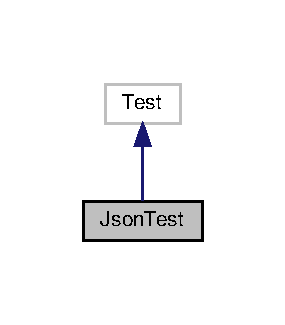
\includegraphics[width=137pt]{classJsonTest__inherit__graph}
\end{center}
\end{figure}


Collaboration diagram for Json\+Test\+:\nopagebreak
\begin{figure}[H]
\begin{center}
\leavevmode
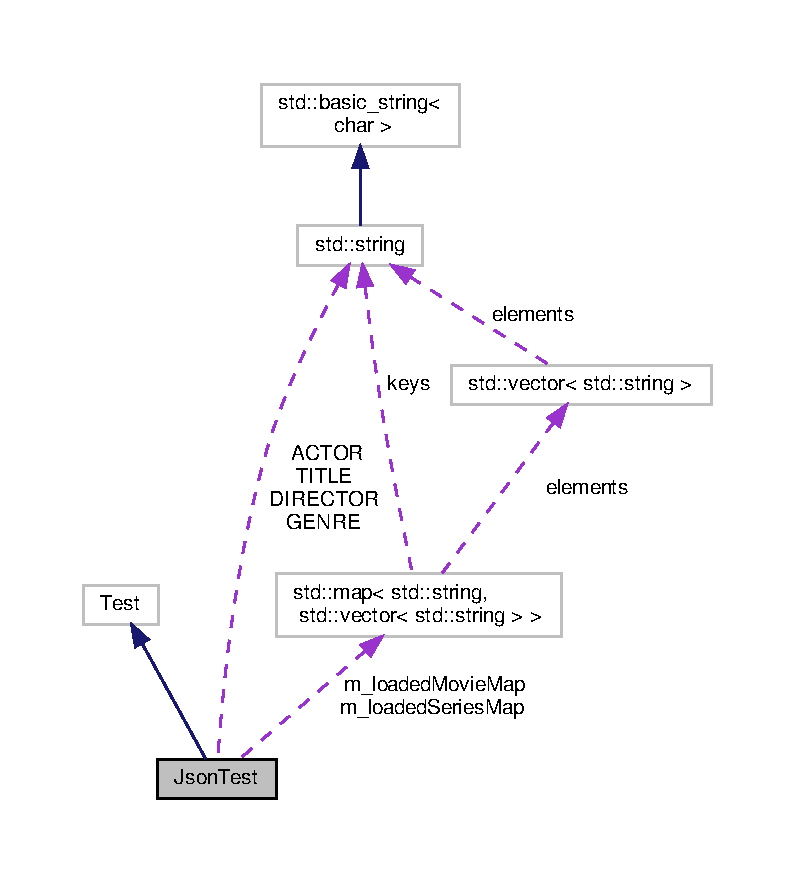
\includegraphics[width=350pt]{classJsonTest__coll__graph}
\end{center}
\end{figure}
\subsection*{Protected Member Functions}
\begin{DoxyCompactItemize}
\item 
\mbox{\Hypertarget{classJsonTest_ae1bbf1b5b144a716ad8b4caefe799654}\label{classJsonTest_ae1bbf1b5b144a716ad8b4caefe799654}} 
void {\bfseries Set\+Up} () override
\item 
\mbox{\Hypertarget{classJsonTest_adc7b6de10eb8ef1552ec09795a9b0769}\label{classJsonTest_adc7b6de10eb8ef1552ec09795a9b0769}} 
void {\bfseries Tear\+Down} () override
\end{DoxyCompactItemize}
\subsection*{Protected Attributes}
\begin{DoxyCompactItemize}
\item 
\mbox{\Hypertarget{classJsonTest_a6e82eb046e59feedc8fcfc109217bf88}\label{classJsonTest_a6e82eb046e59feedc8fcfc109217bf88}} 
std\+::map$<$ std\+::string, std\+::vector$<$ std\+::string $>$ $>$ {\bfseries m\+\_\+loaded\+Movie\+Map}
\item 
\mbox{\Hypertarget{classJsonTest_aa3c7abcfb485941ad83f24253bc961d7}\label{classJsonTest_aa3c7abcfb485941ad83f24253bc961d7}} 
std\+::map$<$ std\+::string, std\+::vector$<$ std\+::string $>$ $>$ {\bfseries m\+\_\+loaded\+Series\+Map}
\item 
\mbox{\Hypertarget{classJsonTest_aa86a225b926154680154c0a884e30b8a}\label{classJsonTest_aa86a225b926154680154c0a884e30b8a}} 
const std\+::string {\bfseries T\+I\+T\+LE} = \char`\"{}title\char`\"{}
\item 
\mbox{\Hypertarget{classJsonTest_ae09f5bfffe12fdd795c4d6d60c14368b}\label{classJsonTest_ae09f5bfffe12fdd795c4d6d60c14368b}} 
const std\+::string {\bfseries G\+E\+N\+RE} = \char`\"{}genre\char`\"{}
\item 
\mbox{\Hypertarget{classJsonTest_a7226a1a843bcd13ff167ec9d07783f81}\label{classJsonTest_a7226a1a843bcd13ff167ec9d07783f81}} 
const std\+::string {\bfseries A\+C\+T\+OR} = \char`\"{}actor\char`\"{}
\item 
\mbox{\Hypertarget{classJsonTest_a991fb6a3ee4f8511b4624334f47b1b56}\label{classJsonTest_a991fb6a3ee4f8511b4624334f47b1b56}} 
const std\+::string {\bfseries D\+I\+R\+E\+C\+T\+OR} = \char`\"{}director\char`\"{}
\end{DoxyCompactItemize}


The documentation for this class was generated from the following file\+:\begin{DoxyCompactItemize}
\item 
inc/unittests/Test\+\_\+\+Json.\+h\end{DoxyCompactItemize}

\hypertarget{classLogger}{}\section{Logger Class Reference}
\label{classLogger}\index{Logger@{Logger}}


Inheritance diagram for Logger\+:\nopagebreak
\begin{figure}[H]
\begin{center}
\leavevmode
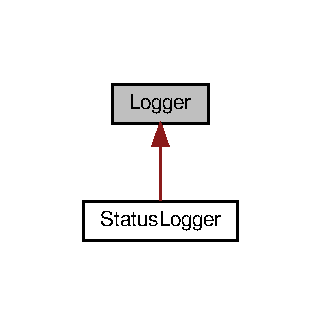
\includegraphics[width=154pt]{classLogger__inherit__graph}
\end{center}
\end{figure}


Collaboration diagram for Logger\+:\nopagebreak
\begin{figure}[H]
\begin{center}
\leavevmode
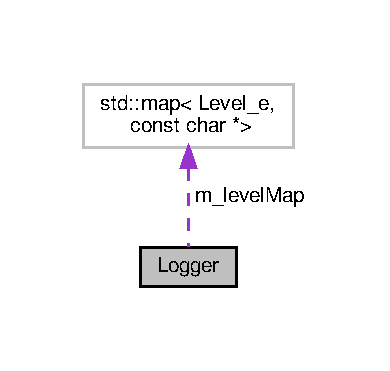
\includegraphics[width=187pt]{classLogger__coll__graph}
\end{center}
\end{figure}
\subsection*{Classes}
\begin{DoxyCompactItemize}
\item 
struct \hyperlink{structLogger_1_1map__init__helper}{map\+\_\+init\+\_\+helper}
\end{DoxyCompactItemize}
\subsection*{Public Types}
\begin{DoxyCompactItemize}
\item 
\mbox{\Hypertarget{classLogger_aa1875ace78bce45b33f84d7f5de7790d}\label{classLogger_aa1875ace78bce45b33f84d7f5de7790d}} 
enum {\bfseries Level\+\_\+e} \{ {\bfseries I\+N\+FO} = 0, 
{\bfseries E\+RR} = 1, 
{\bfseries W\+A\+RN} = 2
 \}
\end{DoxyCompactItemize}
\subsection*{Public Member Functions}
\begin{DoxyCompactItemize}
\item 
\mbox{\Hypertarget{classLogger_a60f8d2a66d45b0ae89aeb59186bb6c0a}\label{classLogger_a60f8d2a66d45b0ae89aeb59186bb6c0a}} 
virtual void {\bfseries T\+R\+A\+CE} (Level\+\_\+e level, std\+::string message, std\+::string error\+Code)=0
\item 
\mbox{\Hypertarget{classLogger_acff1531ccd76c30d960e600eac3de005}\label{classLogger_acff1531ccd76c30d960e600eac3de005}} 
virtual void {\bfseries T\+R\+A\+CE} (Level\+\_\+e level, std\+::string message)=0
\end{DoxyCompactItemize}
\subsection*{Public Attributes}
\begin{DoxyCompactItemize}
\item 
\mbox{\Hypertarget{classLogger_a5e3acb7eae07a5cee57d28711ce45413}\label{classLogger_a5e3acb7eae07a5cee57d28711ce45413}} 
std\+::map$<$ Level\+\_\+e, const char $\ast$ $>$ {\bfseries m\+\_\+level\+Map}
\end{DoxyCompactItemize}
\subsection*{Static Public Attributes}
\begin{DoxyCompactItemize}
\item 
\mbox{\Hypertarget{classLogger_ade70cee1c967259b5dc2448424c7df68}\label{classLogger_ade70cee1c967259b5dc2448424c7df68}} 
static enum Logger\+::\+Level\+\_\+e {\bfseries level}
\end{DoxyCompactItemize}
\subsection*{Protected Member Functions}
\begin{DoxyCompactItemize}
\item 
\mbox{\Hypertarget{classLogger_ac05df84a2b15ca6e1b3b6119a3b7a32c}\label{classLogger_ac05df84a2b15ca6e1b3b6119a3b7a32c}} 
std\+::string {\bfseries get\+Date} ()
\item 
\mbox{\Hypertarget{classLogger_af6e809c7f6fe8d2f829ce0d6a760e0ce}\label{classLogger_af6e809c7f6fe8d2f829ce0d6a760e0ce}} 
std\+::string {\bfseries get\+Time} ()
\item 
\mbox{\Hypertarget{classLogger_a8416f3e0b6fa98d42ca890c0577dff34}\label{classLogger_a8416f3e0b6fa98d42ca890c0577dff34}} 
{\footnotesize template$<$typename T $>$ }\\\hyperlink{structLogger_1_1map__init__helper}{map\+\_\+init\+\_\+helper}$<$ T $>$ {\bfseries map\+\_\+init} (T \&item)
\end{DoxyCompactItemize}


The documentation for this class was generated from the following file\+:\begin{DoxyCompactItemize}
\item 
inc/ifc/Logger.\+h\end{DoxyCompactItemize}

\hypertarget{structLogger_1_1map__init__helper}{}\section{Logger\+:\+:map\+\_\+init\+\_\+helper$<$ T $>$ Struct Template Reference}
\label{structLogger_1_1map__init__helper}\index{Logger\+::map\+\_\+init\+\_\+helper$<$ T $>$@{Logger\+::map\+\_\+init\+\_\+helper$<$ T $>$}}
\subsection*{Public Member Functions}
\begin{DoxyCompactItemize}
\item 
\mbox{\Hypertarget{structLogger_1_1map__init__helper_a64b7b9158fe41bd43498bf2b2707d612}\label{structLogger_1_1map__init__helper_a64b7b9158fe41bd43498bf2b2707d612}} 
{\bfseries map\+\_\+init\+\_\+helper} (T \&d)
\item 
\mbox{\Hypertarget{structLogger_1_1map__init__helper_aa48a30eac8bebde37fff11b69426b27a}\label{structLogger_1_1map__init__helper_aa48a30eac8bebde37fff11b69426b27a}} 
\hyperlink{structLogger_1_1map__init__helper}{map\+\_\+init\+\_\+helper} \& {\bfseries operator()} (typename T\+::key\+\_\+type const \&key, typename T\+::mapped\+\_\+type const \&value)
\end{DoxyCompactItemize}
\subsection*{Public Attributes}
\begin{DoxyCompactItemize}
\item 
\mbox{\Hypertarget{structLogger_1_1map__init__helper_afa0d45b9ba41fd2e55e4eb8aa3c9377e}\label{structLogger_1_1map__init__helper_afa0d45b9ba41fd2e55e4eb8aa3c9377e}} 
T \& {\bfseries data}
\end{DoxyCompactItemize}


The documentation for this struct was generated from the following file\+:\begin{DoxyCompactItemize}
\item 
inc/ifc/Logger.\+h\end{DoxyCompactItemize}

\hypertarget{classMediaHandler}{}\section{Media\+Handler Class Reference}
\label{classMediaHandler}\index{Media\+Handler@{Media\+Handler}}


Synchronizes information from server and database, Implements observer pattern.  




Inheritance diagram for Media\+Handler\+:\nopagebreak
\begin{figure}[H]
\begin{center}
\leavevmode
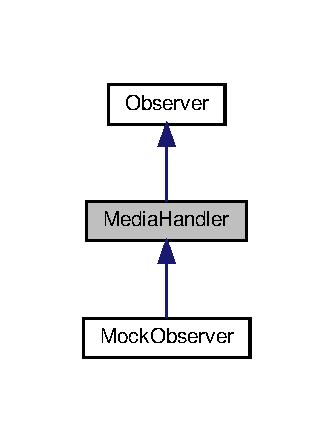
\includegraphics[width=160pt]{classMediaHandler__inherit__graph}
\end{center}
\end{figure}


Collaboration diagram for Media\+Handler\+:\nopagebreak
\begin{figure}[H]
\begin{center}
\leavevmode
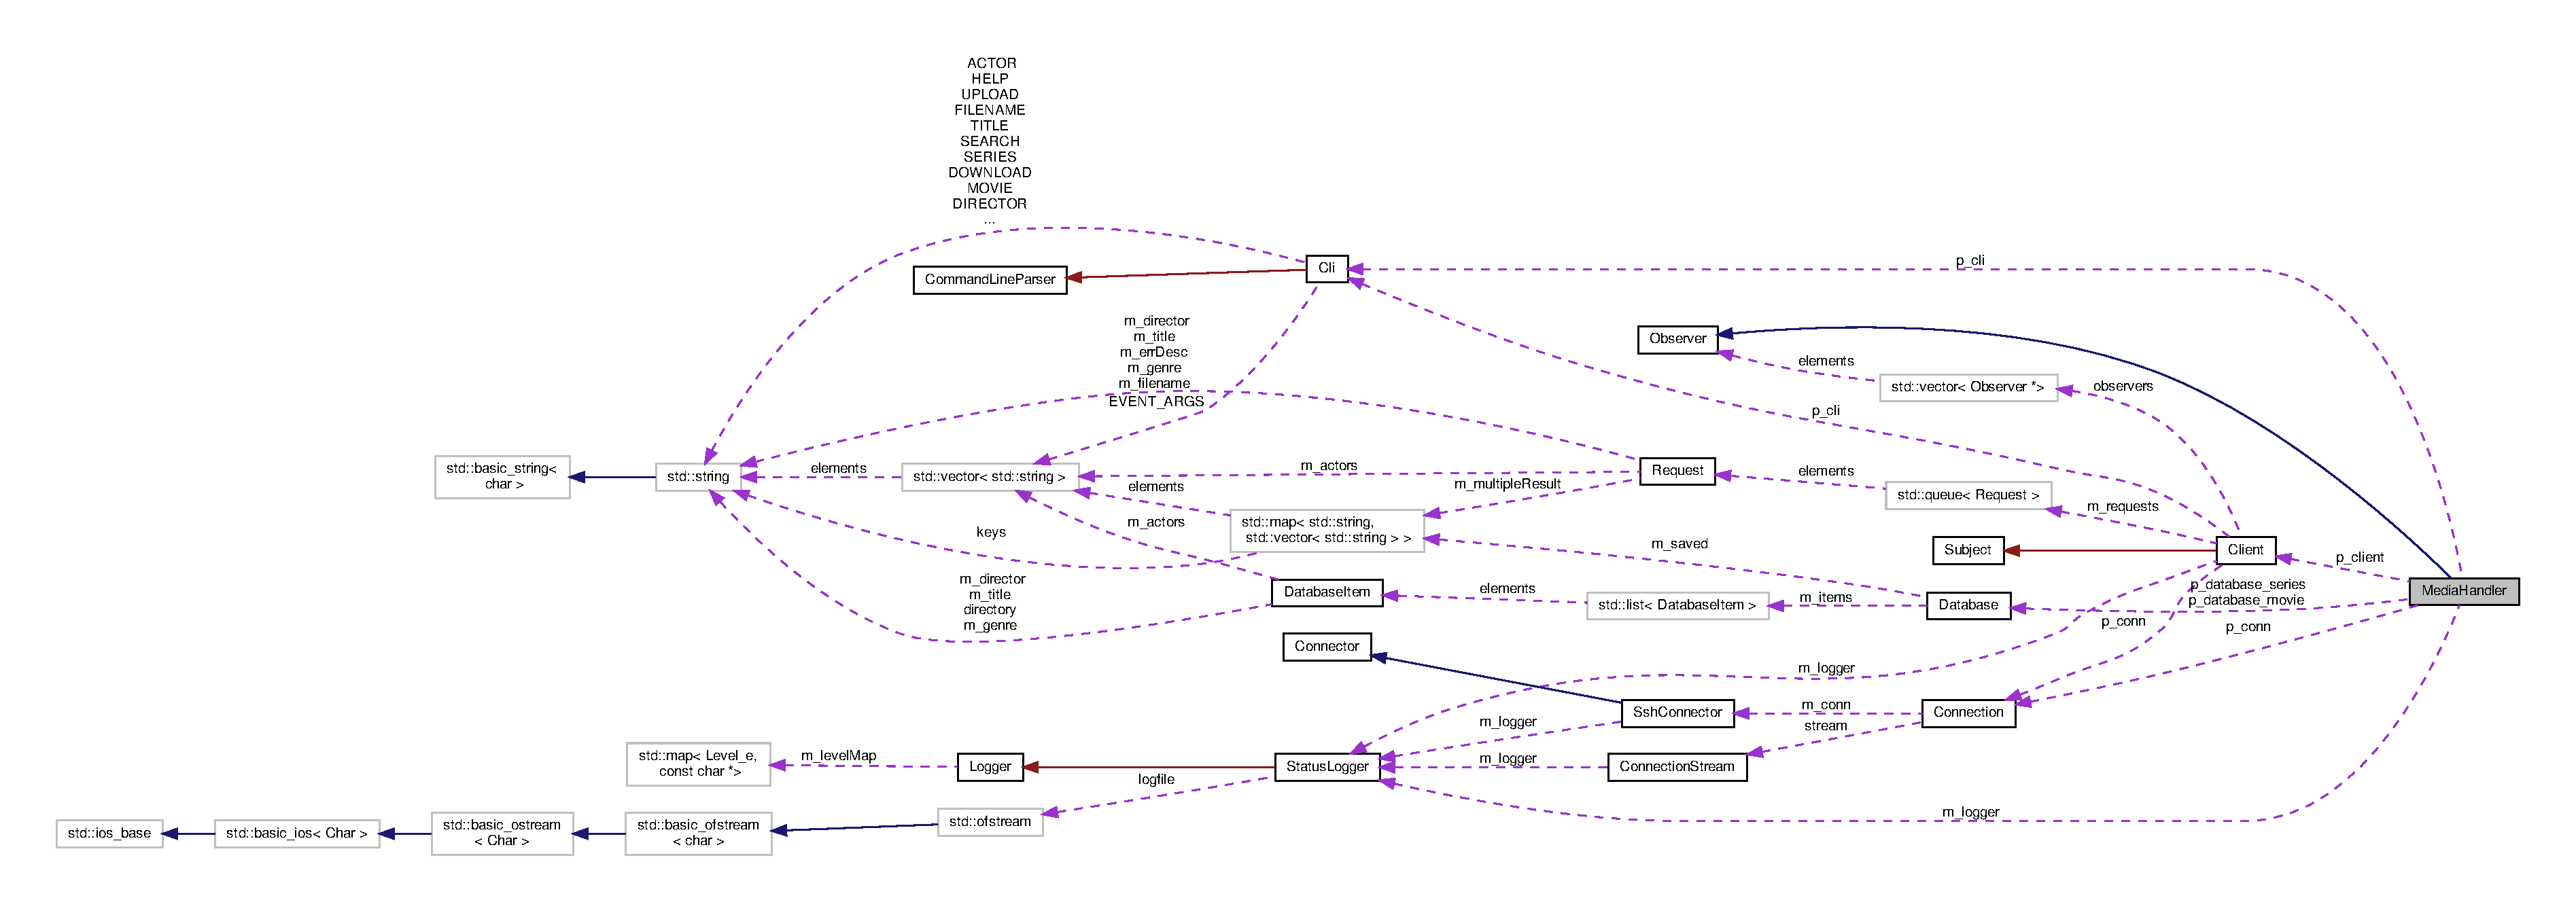
\includegraphics[width=350pt]{classMediaHandler__coll__graph}
\end{center}
\end{figure}
\subsection*{Public Member Functions}
\begin{DoxyCompactItemize}
\item 
\mbox{\Hypertarget{classMediaHandler_ad244cb53ebdabf58f2c54d5cb418f0cb}\label{classMediaHandler_ad244cb53ebdabf58f2c54d5cb418f0cb}} 
{\bfseries Media\+Handler} (Category \&category)
\item 
int \hyperlink{classMediaHandler_ae0c5fa9c02ac287d2e04699d67a02eaf}{update} (\hyperlink{classRequest}{Request} \&request) override
\begin{DoxyCompactList}\small\item\em receives new request from client \end{DoxyCompactList}\item 
\mbox{\Hypertarget{classMediaHandler_a2cb06c3f6c1bd1af74ab4692723c89f6}\label{classMediaHandler_a2cb06c3f6c1bd1af74ab4692723c89f6}} 
void {\bfseries start\+Threads} ()
\end{DoxyCompactItemize}
\subsection*{Public Attributes}
\begin{DoxyCompactItemize}
\item 
\mbox{\Hypertarget{classMediaHandler_aba19c2fd2e904d928ce5914f9dbf8f38}\label{classMediaHandler_aba19c2fd2e904d928ce5914f9dbf8f38}} 
\hyperlink{classClient}{Client} $\ast$ {\bfseries p\+\_\+client}
\end{DoxyCompactItemize}
\subsection*{Private Types}
\begin{DoxyCompactItemize}
\item 
\mbox{\Hypertarget{classMediaHandler_a37ef6d69a0f149af8df7166f43882721}\label{classMediaHandler_a37ef6d69a0f149af8df7166f43882721}} 
enum {\bfseries Status} \{ \newline
{\bfseries D\+O\+W\+N\+L\+O\+A\+D\+I\+NG} = 0, 
{\bfseries U\+P\+L\+O\+A\+D\+I\+NG}, 
{\bfseries S\+T\+R\+E\+A\+M\+I\+NG} = 2, 
{\bfseries S\+E\+A\+R\+C\+H\+I\+NG}, 
\newline
{\bfseries D\+E\+L\+E\+T\+I\+NG}, 
{\bfseries I\+D\+LE}, 
{\bfseries D\+I\+S\+C\+O\+N\+N\+E\+CT}
 \}
\end{DoxyCompactItemize}
\subsection*{Private Member Functions}
\begin{DoxyCompactItemize}
\item 
\mbox{\Hypertarget{classMediaHandler_ad8e1965db78ff745b98cbd21384ac11f}\label{classMediaHandler_ad8e1965db78ff745b98cbd21384ac11f}} 
void {\bfseries sync\+Database} (const \hyperlink{classRequest}{Request} \&request)
\item 
\mbox{\Hypertarget{classMediaHandler_a66c822377acfe8f8dcf3d1de6e15b742}\label{classMediaHandler_a66c822377acfe8f8dcf3d1de6e15b742}} 
void {\bfseries get\+Connection\+Info} (Event \&event, Progress \&progress)
\end{DoxyCompactItemize}
\subsection*{Static Private Member Functions}
\begin{DoxyCompactItemize}
\item 
\mbox{\Hypertarget{classMediaHandler_a6d000e049af4e966f14e131f94776ad0}\label{classMediaHandler_a6d000e049af4e966f14e131f94776ad0}} 
static Status {\bfseries update\+Database\+Info} (const \hyperlink{classRequest}{Request} \&request)
\end{DoxyCompactItemize}
\subsection*{Private Attributes}
\begin{DoxyCompactItemize}
\item 
\mbox{\Hypertarget{classMediaHandler_a51ea5ce2402007e0f7071c7f15b1801a}\label{classMediaHandler_a51ea5ce2402007e0f7071c7f15b1801a}} 
\hyperlink{classStatusLogger}{Status\+Logger} $\ast$ {\bfseries m\+\_\+logger}
\item 
\mbox{\Hypertarget{classMediaHandler_aaf8cff20c4b878940dc7541634e8b0bc}\label{classMediaHandler_aaf8cff20c4b878940dc7541634e8b0bc}} 
\hyperlink{classConnection}{Connection} $\ast$ {\bfseries p\+\_\+conn}
\item 
\mbox{\Hypertarget{classMediaHandler_a2911148d911d30a1d440aca4b13277bf}\label{classMediaHandler_a2911148d911d30a1d440aca4b13277bf}} 
\hyperlink{classCli}{Cli} $\ast$ {\bfseries p\+\_\+cli}
\item 
\mbox{\Hypertarget{classMediaHandler_a41a2bafa6e5b6b1de2f23e7a74581e91}\label{classMediaHandler_a41a2bafa6e5b6b1de2f23e7a74581e91}} 
\hyperlink{classDatabase}{Database} $\ast$ {\bfseries p\+\_\+database\+\_\+movie}
\item 
\mbox{\Hypertarget{classMediaHandler_aa79a92717b0ff21c5375a6eb107543cf}\label{classMediaHandler_aa79a92717b0ff21c5375a6eb107543cf}} 
\hyperlink{classDatabase}{Database} $\ast$ {\bfseries p\+\_\+database\+\_\+series}
\item 
\mbox{\Hypertarget{classMediaHandler_a91120003da62a4022819235d391bd8b6}\label{classMediaHandler_a91120003da62a4022819235d391bd8b6}} 
enum Media\+Handler\+::\+Status {\bfseries status}
\end{DoxyCompactItemize}


\subsection{Detailed Description}
Synchronizes information from server and database, Implements observer pattern. 

for a user instance 

\subsection{Member Function Documentation}
\mbox{\Hypertarget{classMediaHandler_ae0c5fa9c02ac287d2e04699d67a02eaf}\label{classMediaHandler_ae0c5fa9c02ac287d2e04699d67a02eaf}} 
\index{Media\+Handler@{Media\+Handler}!update@{update}}
\index{update@{update}!Media\+Handler@{Media\+Handler}}
\subsubsection{\texorpdfstring{update()}{update()}}
{\footnotesize\ttfamily int Media\+Handler\+::update (\begin{DoxyParamCaption}\item[{\hyperlink{classRequest}{Request} \&}]{request }\end{DoxyParamCaption})\hspace{0.3cm}{\ttfamily [override]}, {\ttfamily [virtual]}}



receives new request from client 

\hyperlink{classMediaHandler_ae0c5fa9c02ac287d2e04699d67a02eaf}{Media\+Handler\+::update} method update 
\begin{DoxyParams}{Parameters}
{\em request} & \\
\hline
\end{DoxyParams}
\begin{DoxyReturn}{Returns}

\end{DoxyReturn}


Implements \hyperlink{classObserver_acc79119027d8770fe4946161d6274a00}{Observer}.



The documentation for this class was generated from the following files\+:\begin{DoxyCompactItemize}
\item 
inc/Media\+Handler.\+h\item 
src/Media\+Handler.\+cpp\end{DoxyCompactItemize}

\hypertarget{classMockObserver}{}\section{Mock\+Observer Class Reference}
\label{classMockObserver}\index{Mock\+Observer@{Mock\+Observer}}


Inheritance diagram for Mock\+Observer\+:\nopagebreak
\begin{figure}[H]
\begin{center}
\leavevmode
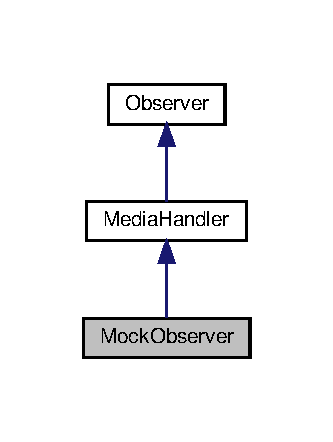
\includegraphics[width=160pt]{classMockObserver__inherit__graph}
\end{center}
\end{figure}


Collaboration diagram for Mock\+Observer\+:\nopagebreak
\begin{figure}[H]
\begin{center}
\leavevmode
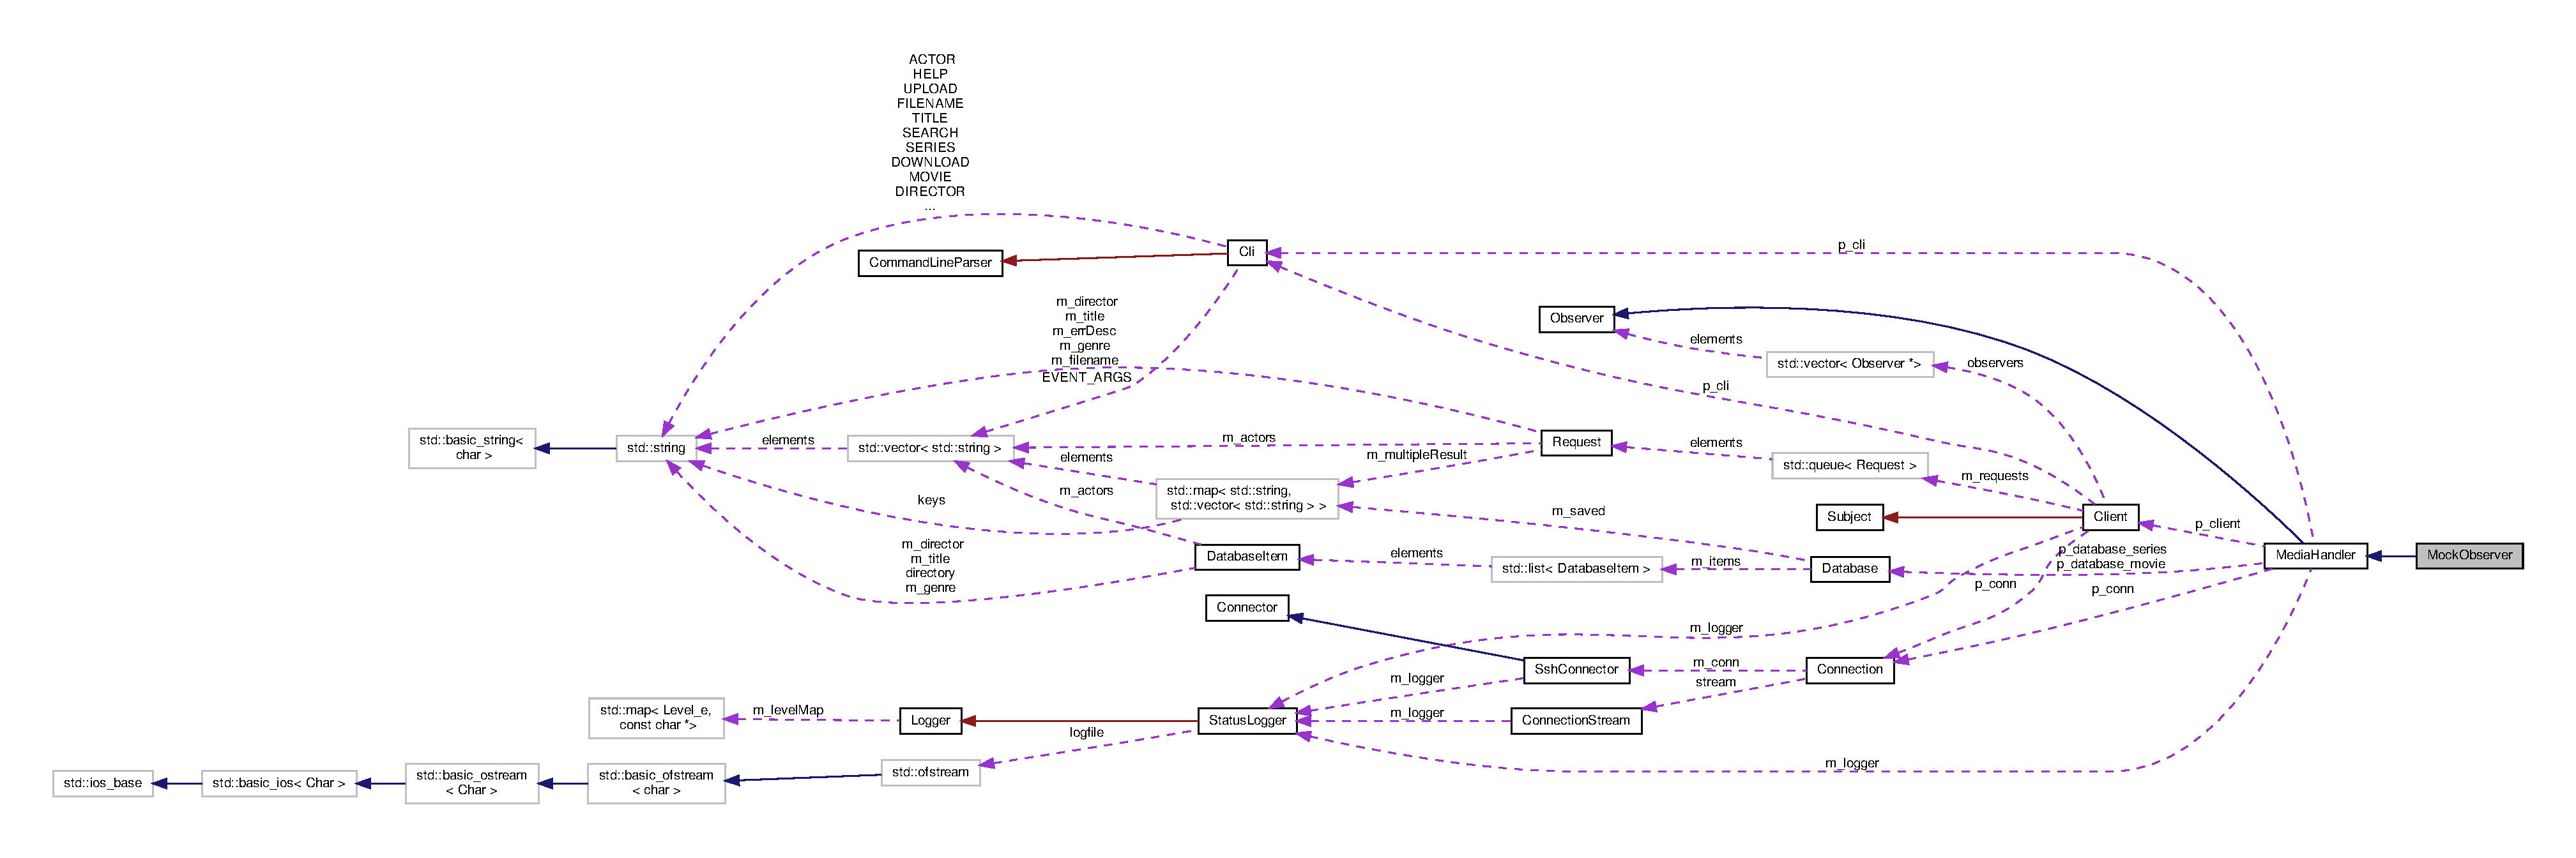
\includegraphics[width=350pt]{classMockObserver__coll__graph}
\end{center}
\end{figure}
\subsection*{Public Member Functions}
\begin{DoxyCompactItemize}
\item 
\mbox{\Hypertarget{classMockObserver_a9e5d475e1c41dff9f789c8c9daf50de8}\label{classMockObserver_a9e5d475e1c41dff9f789c8c9daf50de8}} 
{\bfseries M\+O\+C\+K\+\_\+\+M\+E\+T\+H\+O\+D1} (\hyperlink{classMediaHandler_ae0c5fa9c02ac287d2e04699d67a02eaf}{update}, int(\hyperlink{classRequest}{Request} \&))
\item 
int \hyperlink{classMediaHandler_ae0c5fa9c02ac287d2e04699d67a02eaf}{update} (\hyperlink{classRequest}{Request} \&request) override
\begin{DoxyCompactList}\small\item\em receives new request from client \end{DoxyCompactList}\item 
\mbox{\Hypertarget{classMediaHandler_a2cb06c3f6c1bd1af74ab4692723c89f6}\label{classMediaHandler_a2cb06c3f6c1bd1af74ab4692723c89f6}} 
void {\bfseries start\+Threads} ()
\end{DoxyCompactItemize}
\subsection*{Public Attributes}
\begin{DoxyCompactItemize}
\item 
\mbox{\Hypertarget{classMediaHandler_aba19c2fd2e904d928ce5914f9dbf8f38}\label{classMediaHandler_aba19c2fd2e904d928ce5914f9dbf8f38}} 
\hyperlink{classClient}{Client} $\ast$ {\bfseries p\+\_\+client}
\end{DoxyCompactItemize}


\subsection{Member Function Documentation}
\mbox{\Hypertarget{classMediaHandler_ae0c5fa9c02ac287d2e04699d67a02eaf}\label{classMediaHandler_ae0c5fa9c02ac287d2e04699d67a02eaf}} 
\index{Mock\+Observer@{Mock\+Observer}!update@{update}}
\index{update@{update}!Mock\+Observer@{Mock\+Observer}}
\subsubsection{\texorpdfstring{update()}{update()}}
{\footnotesize\ttfamily int Media\+Handler\+::update (\begin{DoxyParamCaption}\item[{\hyperlink{classRequest}{Request} \&}]{request }\end{DoxyParamCaption})\hspace{0.3cm}{\ttfamily [override]}, {\ttfamily [virtual]}, {\ttfamily [inherited]}}



receives new request from client 

\hyperlink{classMediaHandler_ae0c5fa9c02ac287d2e04699d67a02eaf}{Media\+Handler\+::update} method update 
\begin{DoxyParams}{Parameters}
{\em request} & \\
\hline
\end{DoxyParams}
\begin{DoxyReturn}{Returns}

\end{DoxyReturn}


Implements \hyperlink{classObserver_acc79119027d8770fe4946161d6274a00}{Observer}.



The documentation for this class was generated from the following file\+:\begin{DoxyCompactItemize}
\item 
inc/unittests/Test\+\_\+\+Observer.\+h\end{DoxyCompactItemize}

\hypertarget{classMovieDatabase}{}\section{Movie\+Database Class Reference}
\label{classMovieDatabase}\index{Movie\+Database@{Movie\+Database}}


A module that implements the functionality of \hyperlink{Database_8h_source}{Database.\+h} and helps the client to perform database actions.  




{\ttfamily \#include $<$Movie\+Database.\+h$>$}



Inheritance diagram for Movie\+Database\+:
\nopagebreak
\begin{figure}[H]
\begin{center}
\leavevmode
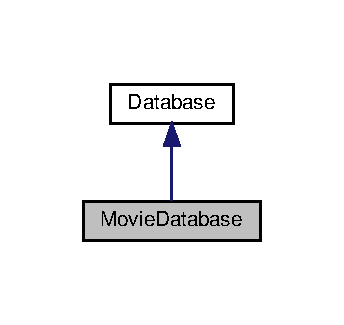
\includegraphics[width=172pt]{classMovieDatabase__inherit__graph}
\end{center}
\end{figure}


Collaboration diagram for Movie\+Database\+:
\nopagebreak
\begin{figure}[H]
\begin{center}
\leavevmode
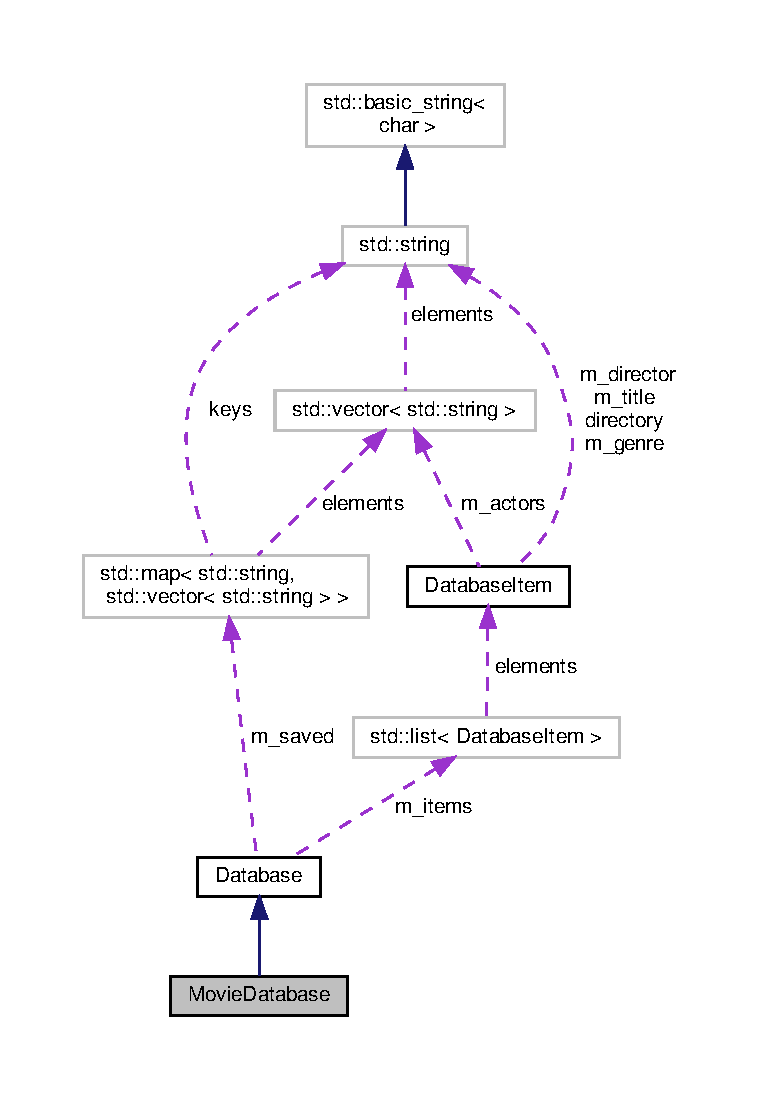
\includegraphics[width=350pt]{classMovieDatabase__coll__graph}
\end{center}
\end{figure}
\subsection*{Public Member Functions}
\begin{DoxyCompactItemize}
\item 
void \hyperlink{classMovieDatabase_a203b9b5c1b325997ce519859a436b6ce}{push\+Item} (const \hyperlink{classDatabaseItem}{Database\+Item} \&m\+\_\+item) override
\begin{DoxyCompactList}\small\item\em Implementation for virtual member of \hyperlink{Database_8h_source}{Database.\+h} Uploads the requested database item. \end{DoxyCompactList}\item 
\hyperlink{classDatabaseItem}{Database\+Item} \hyperlink{classMovieDatabase_ac0bb39b8be599ffea76081809ae42dda}{fetch\+Item} (const std\+::string \&title) override
\begin{DoxyCompactList}\small\item\em Implementation for virtual member of \hyperlink{Database_8h_source}{Database.\+h} Fetch the requested database item. \end{DoxyCompactList}\item 
long \hyperlink{classMovieDatabase_a9a386f51dd72d63414a124cbcfcd879b}{get\+Number\+Of\+Item} () override
\begin{DoxyCompactList}\small\item\em Implementation for virtual member of \hyperlink{Database_8h_source}{Database.\+h} Method that return the size of the database. \end{DoxyCompactList}\item 
void \hyperlink{classMovieDatabase_a85faa4c33b3ab2dc0d1f4939bb034797}{purge\+Item} (const \hyperlink{classDatabaseItem}{Database\+Item} \&m\+\_\+item) override
\begin{DoxyCompactList}\small\item\em Implementation for virtual member of \hyperlink{Database_8h_source}{Database.\+h} Delete the requested database item. \end{DoxyCompactList}\item 
void \hyperlink{classMovieDatabase_af1e13b6fc0fd7186e98edbe2cf187618}{print\+All} () override
\begin{DoxyCompactList}\small\item\em Implementation for virtual member of \hyperlink{Database_8h_source}{Database.\+h} Prints the entire database content. \end{DoxyCompactList}\end{DoxyCompactItemize}
\subsection*{Additional Inherited Members}


\subsection{Detailed Description}
A module that implements the functionality of \hyperlink{Database_8h_source}{Database.\+h} and helps the client to perform database actions. 



\subsection{Member Function Documentation}
\mbox{\Hypertarget{classMovieDatabase_ac0bb39b8be599ffea76081809ae42dda}\label{classMovieDatabase_ac0bb39b8be599ffea76081809ae42dda}} 
\index{Movie\+Database@{Movie\+Database}!fetch\+Item@{fetch\+Item}}
\index{fetch\+Item@{fetch\+Item}!Movie\+Database@{Movie\+Database}}
\subsubsection{\texorpdfstring{fetch\+Item()}{fetchItem()}}
{\footnotesize\ttfamily \hyperlink{classDatabaseItem}{Database\+Item} Movie\+Database\+::fetch\+Item (\begin{DoxyParamCaption}\item[{const std\+::string \&}]{title }\end{DoxyParamCaption})\hspace{0.3cm}{\ttfamily [inline]}, {\ttfamily [override]}, {\ttfamily [virtual]}}



Implementation for virtual member of \hyperlink{Database_8h_source}{Database.\+h} Fetch the requested database item. 

A const reference to a title

\begin{DoxyReturn}{Returns}
The requested \hyperlink{classDatabaseItem}{Database\+Item}
\end{DoxyReturn}


Reimplemented from \hyperlink{classDatabase_a40254eec69c7d7cc15da24a9f0b072b3}{Database}.

\mbox{\Hypertarget{classMovieDatabase_a9a386f51dd72d63414a124cbcfcd879b}\label{classMovieDatabase_a9a386f51dd72d63414a124cbcfcd879b}} 
\index{Movie\+Database@{Movie\+Database}!get\+Number\+Of\+Item@{get\+Number\+Of\+Item}}
\index{get\+Number\+Of\+Item@{get\+Number\+Of\+Item}!Movie\+Database@{Movie\+Database}}
\subsubsection{\texorpdfstring{get\+Number\+Of\+Item()}{getNumberOfItem()}}
{\footnotesize\ttfamily long Movie\+Database\+::get\+Number\+Of\+Item (\begin{DoxyParamCaption}{ }\end{DoxyParamCaption})\hspace{0.3cm}{\ttfamily [inline]}, {\ttfamily [override]}, {\ttfamily [virtual]}}



Implementation for virtual member of \hyperlink{Database_8h_source}{Database.\+h} Method that return the size of the database. 

\begin{DoxyReturn}{Returns}
Size of the database (long).
\end{DoxyReturn}


Reimplemented from \hyperlink{classDatabase_a230225cb341eb23a99a83ef3d1abae53}{Database}.

\mbox{\Hypertarget{classMovieDatabase_af1e13b6fc0fd7186e98edbe2cf187618}\label{classMovieDatabase_af1e13b6fc0fd7186e98edbe2cf187618}} 
\index{Movie\+Database@{Movie\+Database}!print\+All@{print\+All}}
\index{print\+All@{print\+All}!Movie\+Database@{Movie\+Database}}
\subsubsection{\texorpdfstring{print\+All()}{printAll()}}
{\footnotesize\ttfamily void Movie\+Database\+::print\+All (\begin{DoxyParamCaption}{ }\end{DoxyParamCaption})\hspace{0.3cm}{\ttfamily [inline]}, {\ttfamily [override]}, {\ttfamily [virtual]}}



Implementation for virtual member of \hyperlink{Database_8h_source}{Database.\+h} Prints the entire database content. 

\begin{DoxyReturn}{Returns}

\end{DoxyReturn}


Reimplemented from \hyperlink{classDatabase_afa345da530fd5c8dfe0c978917cd6049}{Database}.

\mbox{\Hypertarget{classMovieDatabase_a85faa4c33b3ab2dc0d1f4939bb034797}\label{classMovieDatabase_a85faa4c33b3ab2dc0d1f4939bb034797}} 
\index{Movie\+Database@{Movie\+Database}!purge\+Item@{purge\+Item}}
\index{purge\+Item@{purge\+Item}!Movie\+Database@{Movie\+Database}}
\subsubsection{\texorpdfstring{purge\+Item()}{purgeItem()}}
{\footnotesize\ttfamily void Movie\+Database\+::purge\+Item (\begin{DoxyParamCaption}\item[{const \hyperlink{classDatabaseItem}{Database\+Item} \&}]{m\+\_\+item }\end{DoxyParamCaption})\hspace{0.3cm}{\ttfamily [inline]}, {\ttfamily [override]}, {\ttfamily [virtual]}}



Implementation for virtual member of \hyperlink{Database_8h_source}{Database.\+h} Delete the requested database item. 

A const reference to a database item

\begin{DoxyReturn}{Returns}

\end{DoxyReturn}


Reimplemented from \hyperlink{classDatabase_a5d232b9f62079682dd7fe7983b252e5e}{Database}.

\mbox{\Hypertarget{classMovieDatabase_a203b9b5c1b325997ce519859a436b6ce}\label{classMovieDatabase_a203b9b5c1b325997ce519859a436b6ce}} 
\index{Movie\+Database@{Movie\+Database}!push\+Item@{push\+Item}}
\index{push\+Item@{push\+Item}!Movie\+Database@{Movie\+Database}}
\subsubsection{\texorpdfstring{push\+Item()}{pushItem()}}
{\footnotesize\ttfamily void Movie\+Database\+::push\+Item (\begin{DoxyParamCaption}\item[{const \hyperlink{classDatabaseItem}{Database\+Item} \&}]{m\+\_\+item }\end{DoxyParamCaption})\hspace{0.3cm}{\ttfamily [inline]}, {\ttfamily [override]}, {\ttfamily [virtual]}}



Implementation for virtual member of \hyperlink{Database_8h_source}{Database.\+h} Uploads the requested database item. 

A const reference to a database item

\begin{DoxyReturn}{Returns}

\end{DoxyReturn}


Reimplemented from \hyperlink{classDatabase_a80fa14ab9f4deadc9a2ab7493f1919a4}{Database}.



The documentation for this class was generated from the following file\+:\begin{DoxyCompactItemize}
\item 
/home/mjonsson/repo/cpp\+Adv/media\+F\+W/inc/\+Database/Movie\+Database.\+h\end{DoxyCompactItemize}

\hypertarget{classNotImplementedException}{}\section{Not\+Implemented\+Exception Class Reference}
\label{classNotImplementedException}\index{Not\+Implemented\+Exception@{Not\+Implemented\+Exception}}


 




{\ttfamily \#include $<$Database.\+h$>$}



Inheritance diagram for Not\+Implemented\+Exception\+:\nopagebreak
\begin{figure}[H]
\begin{center}
\leavevmode
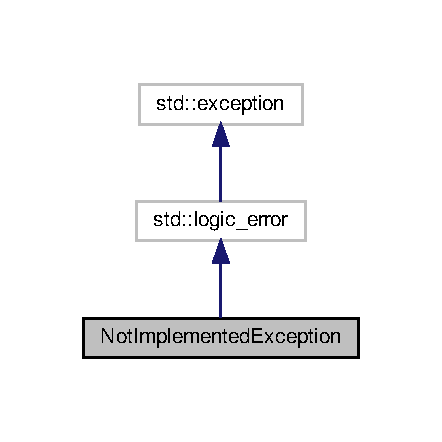
\includegraphics[width=212pt]{classNotImplementedException__inherit__graph}
\end{center}
\end{figure}


Collaboration diagram for Not\+Implemented\+Exception\+:\nopagebreak
\begin{figure}[H]
\begin{center}
\leavevmode
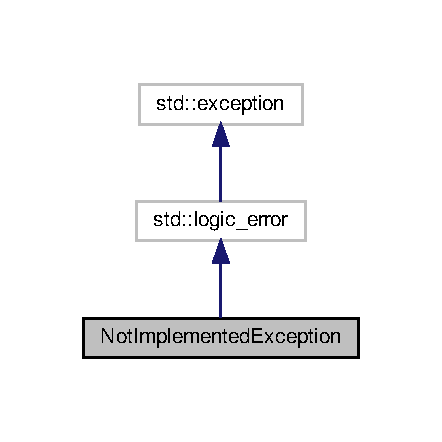
\includegraphics[width=212pt]{classNotImplementedException__coll__graph}
\end{center}
\end{figure}


\subsection{Detailed Description}


A module that works as an interface for subclasses and let them perform database actions 

The documentation for this class was generated from the following file\+:\begin{DoxyCompactItemize}
\item 
inc/database/Database.\+h\end{DoxyCompactItemize}

\hypertarget{classObserver}{}\section{Observer Class Reference}
\label{classObserver}\index{Observer@{Observer}}


Inheritance diagram for Observer\+:\nopagebreak
\begin{figure}[H]
\begin{center}
\leavevmode
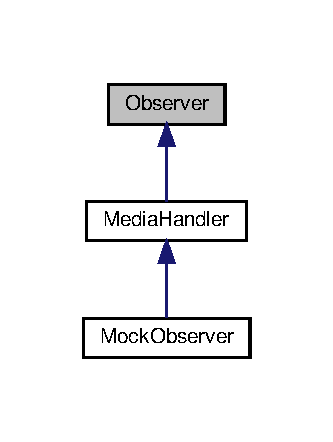
\includegraphics[width=160pt]{classObserver__inherit__graph}
\end{center}
\end{figure}
\subsection*{Public Member Functions}
\begin{DoxyCompactItemize}
\item 
virtual int \hyperlink{classObserver_acc79119027d8770fe4946161d6274a00}{update} (\hyperlink{classRequest}{Request} \&)=0
\end{DoxyCompactItemize}


\subsection{Member Function Documentation}
\mbox{\Hypertarget{classObserver_acc79119027d8770fe4946161d6274a00}\label{classObserver_acc79119027d8770fe4946161d6274a00}} 
\index{Observer@{Observer}!update@{update}}
\index{update@{update}!Observer@{Observer}}
\subsubsection{\texorpdfstring{update()}{update()}}
{\footnotesize\ttfamily virtual int Observer\+::update (\begin{DoxyParamCaption}\item[{\hyperlink{classRequest}{Request} \&}]{ }\end{DoxyParamCaption})\hspace{0.3cm}{\ttfamily [pure virtual]}}

Update the state of this observer 
\begin{DoxyParams}{Parameters}
{\em \hyperlink{classRequest}{Request}} & of update \\
\hline
\end{DoxyParams}


Implemented in \hyperlink{classMediaHandler_ae0c5fa9c02ac287d2e04699d67a02eaf}{Media\+Handler}.



The documentation for this class was generated from the following file\+:\begin{DoxyCompactItemize}
\item 
inc/ifc/Observer.\+h\end{DoxyCompactItemize}

\hypertarget{classObserverTest}{}\section{Observer\+Test Class Reference}
\label{classObserverTest}\index{Observer\+Test@{Observer\+Test}}


Inheritance diagram for Observer\+Test\+:\nopagebreak
\begin{figure}[H]
\begin{center}
\leavevmode
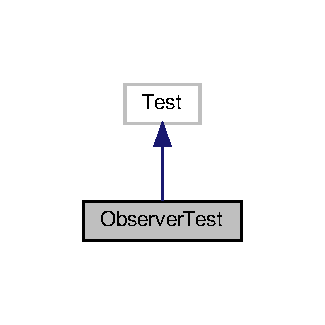
\includegraphics[width=156pt]{classObserverTest__inherit__graph}
\end{center}
\end{figure}


Collaboration diagram for Observer\+Test\+:\nopagebreak
\begin{figure}[H]
\begin{center}
\leavevmode
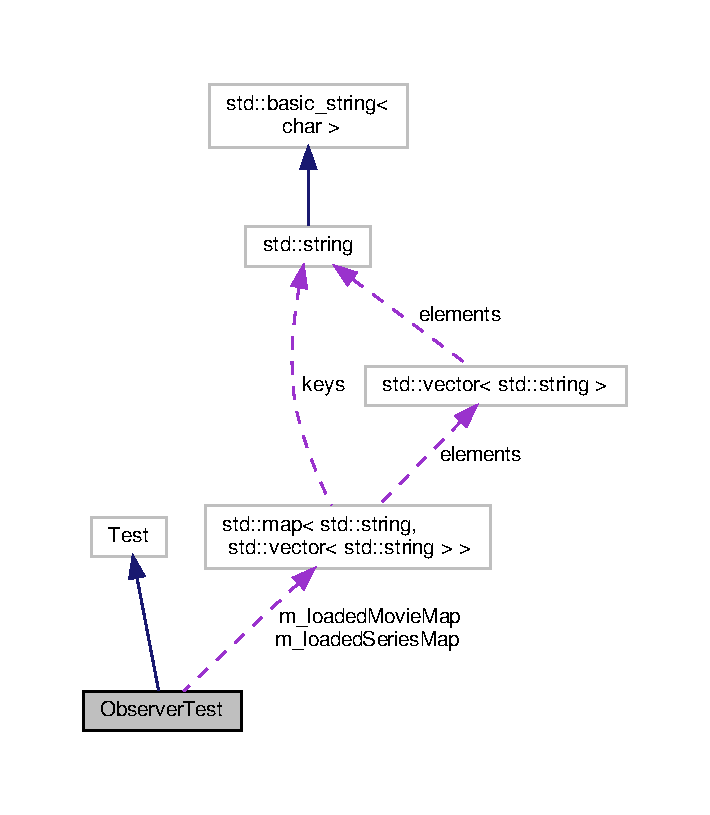
\includegraphics[width=341pt]{classObserverTest__coll__graph}
\end{center}
\end{figure}
\subsection*{Protected Member Functions}
\begin{DoxyCompactItemize}
\item 
\mbox{\Hypertarget{classObserverTest_ab22192ebbb8dc2e7d6f29635108b803a}\label{classObserverTest_ab22192ebbb8dc2e7d6f29635108b803a}} 
void {\bfseries Set\+Up} () override
\item 
\mbox{\Hypertarget{classObserverTest_a8bd0f5cd482a19feb01d8d659e34a4d1}\label{classObserverTest_a8bd0f5cd482a19feb01d8d659e34a4d1}} 
void {\bfseries Tear\+Down} () override
\end{DoxyCompactItemize}
\subsection*{Protected Attributes}
\begin{DoxyCompactItemize}
\item 
\mbox{\Hypertarget{classObserverTest_a033a35884b4b765bf1da7b11b4aba26e}\label{classObserverTest_a033a35884b4b765bf1da7b11b4aba26e}} 
std\+::map$<$ std\+::string, std\+::vector$<$ std\+::string $>$ $>$ {\bfseries m\+\_\+loaded\+Movie\+Map}
\item 
\mbox{\Hypertarget{classObserverTest_accbfbd6967383c6982fe603c077764bb}\label{classObserverTest_accbfbd6967383c6982fe603c077764bb}} 
std\+::map$<$ std\+::string, std\+::vector$<$ std\+::string $>$ $>$ {\bfseries m\+\_\+loaded\+Series\+Map}
\end{DoxyCompactItemize}


The documentation for this class was generated from the following file\+:\begin{DoxyCompactItemize}
\item 
inc/unittests/Test\+\_\+\+Observer.\+h\end{DoxyCompactItemize}

\hypertarget{classParser}{}\section{Parser Class Reference}
\label{classParser}\index{Parser@{Parser}}


Inheritance diagram for Parser\+:\nopagebreak
\begin{figure}[H]
\begin{center}
\leavevmode
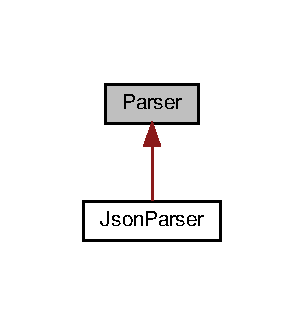
\includegraphics[width=146pt]{classParser__inherit__graph}
\end{center}
\end{figure}
\subsection*{Public Member Functions}
\begin{DoxyCompactItemize}
\item 
\mbox{\Hypertarget{classParser_a81703f49fece0260dc74bdc0ec2f2afe}\label{classParser_a81703f49fece0260dc74bdc0ec2f2afe}} 
virtual void {\bfseries clear} ()=0
\item 
\mbox{\Hypertarget{classParser_a0c7ff57756720984203d88cd98ae59b1}\label{classParser_a0c7ff57756720984203d88cd98ae59b1}} 
virtual void {\bfseries load} (const Category \&category)=0
\item 
\mbox{\Hypertarget{classParser_a370e612b404bf66118d23234cf294e39}\label{classParser_a370e612b404bf66118d23234cf294e39}} 
virtual void {\bfseries add} (const Category \&category, \hyperlink{classDatabaseItem}{Database\+Item} \&item)=0
\item 
\mbox{\Hypertarget{classParser_aa10c06db53b068f2f14de7160d2be927}\label{classParser_aa10c06db53b068f2f14de7160d2be927}} 
virtual void {\bfseries remove} (const Category \&category, \hyperlink{classDatabaseItem}{Database\+Item} \&item)=0
\item 
\mbox{\Hypertarget{classParser_a0fbcf702bd9426dcc15f15900ebb0afb}\label{classParser_a0fbcf702bd9426dcc15f15900ebb0afb}} 
virtual bool {\bfseries find} (Category \&category, const std\+::string \&val)=0
\end{DoxyCompactItemize}


The documentation for this class was generated from the following file\+:\begin{DoxyCompactItemize}
\item 
inc/ifc/Parser.\+h\end{DoxyCompactItemize}

\hypertarget{classRequest}{}\section{Request Class Reference}
\label{classRequest}\index{Request@{Request}}


Collaboration diagram for Request\+:\nopagebreak
\begin{figure}[H]
\begin{center}
\leavevmode
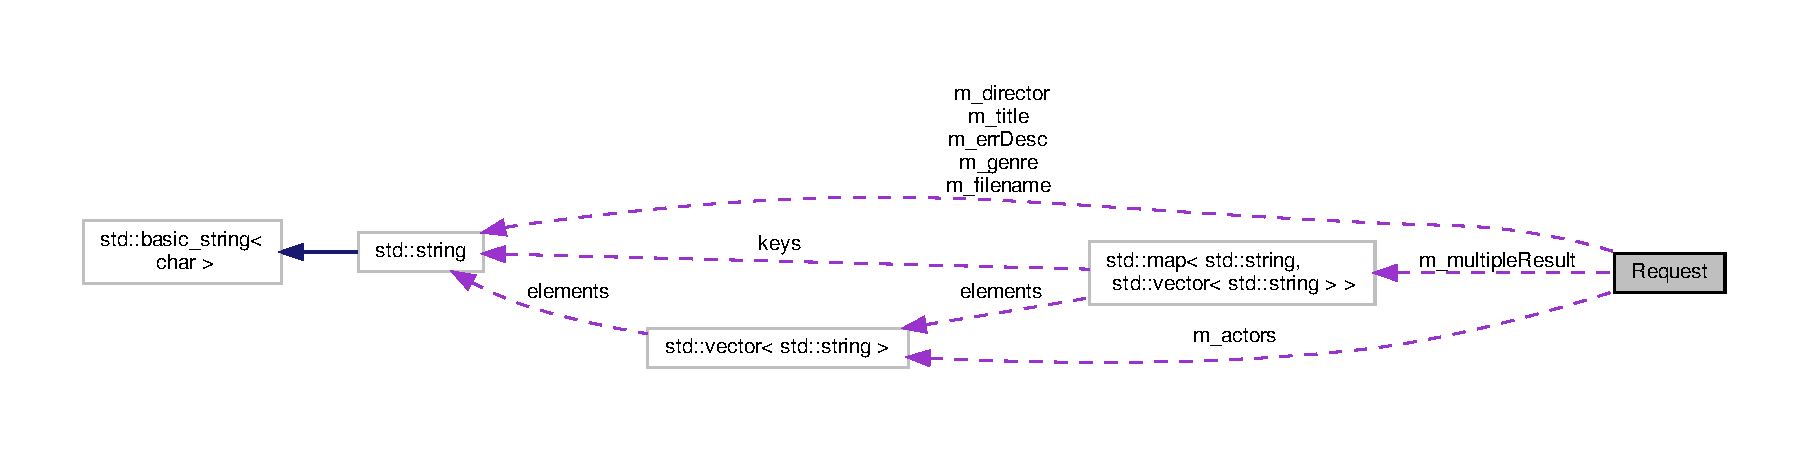
\includegraphics[width=350pt]{classRequest__coll__graph}
\end{center}
\end{figure}
\subsection*{Public Member Functions}
\begin{DoxyCompactItemize}
\item 
\mbox{\Hypertarget{classRequest_a91e125c20f0c1923aeb8af789bb24b84}\label{classRequest_a91e125c20f0c1923aeb8af789bb24b84}} 
{\bfseries Request} (Event \+\_\+event, std\+::string \&\+\_\+title, std\+::string, std\+::string \&\+\_\+genre, std\+::string \&\+\_\+director, std\+::vector$<$ std\+::string $>$ \&\+\_\+actors)
\item 
\mbox{\Hypertarget{classRequest_a4ad527cc19ca9ff74f0a5ad9c668b7d8}\label{classRequest_a4ad527cc19ca9ff74f0a5ad9c668b7d8}} 
{\bfseries Request} (Event \+\_\+event, std\+::string \&\+\_\+title)
\item 
\mbox{\Hypertarget{classRequest_a8c53f5955545d3b4b060eb956858f089}\label{classRequest_a8c53f5955545d3b4b060eb956858f089}} 
{\bfseries Request} (Event \+\_\+event)
\item 
\mbox{\Hypertarget{classRequest_a77b64a169dc4a3383f2266cadfdee50a}\label{classRequest_a77b64a169dc4a3383f2266cadfdee50a}} 
{\bfseries Request} (const int code, const std\+::string desc)
\item 
\mbox{\Hypertarget{classRequest_a580a7d5ebcd266767b79bbcc234227b2}\label{classRequest_a580a7d5ebcd266767b79bbcc234227b2}} 
void {\bfseries set\+Category} (Category cat)
\item 
\mbox{\Hypertarget{classRequest_a1ae3d3d7aa87535e05b69bf64ce3eda6}\label{classRequest_a1ae3d3d7aa87535e05b69bf64ce3eda6}} 
void {\bfseries set\+Progress} (Progress progress)
\item 
\mbox{\Hypertarget{classRequest_a11d39b9c7e5093a5c55cbec0e8beb4fb}\label{classRequest_a11d39b9c7e5093a5c55cbec0e8beb4fb}} 
void {\bfseries set\+Error\+Desc} (const std\+::string \&\+\_\+desc)
\item 
\mbox{\Hypertarget{classRequest_ad0baa58662f3f7883a829b3602d01613}\label{classRequest_ad0baa58662f3f7883a829b3602d01613}} 
void {\bfseries set\+Error} (const int \&\+\_\+err)
\item 
\mbox{\Hypertarget{classRequest_afb77a964fd67486cfa1109c5f45fa240}\label{classRequest_afb77a964fd67486cfa1109c5f45fa240}} 
void {\bfseries set\+Title} (const std\+::string \&\+\_\+title)
\item 
\mbox{\Hypertarget{classRequest_ad11774b94f08627220f093561be85b2a}\label{classRequest_ad11774b94f08627220f093561be85b2a}} 
void {\bfseries set\+Genre} (const std\+::string \&\+\_\+genre)
\item 
\mbox{\Hypertarget{classRequest_af90380270fe528914cd2d7bee34bd987}\label{classRequest_af90380270fe528914cd2d7bee34bd987}} 
void {\bfseries set\+Director} (const std\+::string \&\+\_\+director)
\item 
\mbox{\Hypertarget{classRequest_aab34f8677063f837ad8cca8dda75393a}\label{classRequest_aab34f8677063f837ad8cca8dda75393a}} 
void {\bfseries set\+Actors} (const std\+::vector$<$ std\+::string $>$ \&\+\_\+vec)
\item 
\mbox{\Hypertarget{classRequest_aa18562802f571d76ce3296b3001ffe15}\label{classRequest_aa18562802f571d76ce3296b3001ffe15}} 
void {\bfseries set\+Filename} (const std\+::string \&\+\_\+filename)
\item 
\mbox{\Hypertarget{classRequest_aec880c38436e60224fd02512a9ea3fb7}\label{classRequest_aec880c38436e60224fd02512a9ea3fb7}} 
void {\bfseries set\+Multiple\+Result} (const std\+::map$<$ std\+::string, std\+::vector$<$ std\+::string $>$$>$ \&\+\_\+map)
\item 
\mbox{\Hypertarget{classRequest_afba4fd36f889aec3625a45b7227d318a}\label{classRequest_afba4fd36f889aec3625a45b7227d318a}} 
int {\bfseries get\+Error} ()
\item 
\mbox{\Hypertarget{classRequest_abc555029e5f0bf69bcad19075e444327}\label{classRequest_abc555029e5f0bf69bcad19075e444327}} 
std\+::string {\bfseries get\+Error\+Desc} ()
\item 
\mbox{\Hypertarget{classRequest_aa32770806b75e24aa283b306f3e47552}\label{classRequest_aa32770806b75e24aa283b306f3e47552}} 
Event {\bfseries get\+Event} () const
\item 
\mbox{\Hypertarget{classRequest_ab7046df0d75e35e686f085ddbdebd8f0}\label{classRequest_ab7046df0d75e35e686f085ddbdebd8f0}} 
Progress {\bfseries get\+Progress} ()
\item 
\mbox{\Hypertarget{classRequest_afa4d474657bb1b20a165026317b55018}\label{classRequest_afa4d474657bb1b20a165026317b55018}} 
std\+::string const {\bfseries get\+File\+Name} ()
\item 
\mbox{\Hypertarget{classRequest_a23ed3e91b2a44f5d77404d0c952886d6}\label{classRequest_a23ed3e91b2a44f5d77404d0c952886d6}} 
std\+::string const {\bfseries get\+Title} () const
\item 
\mbox{\Hypertarget{classRequest_a84dfb549a607e1eb8639b1d883dd00d0}\label{classRequest_a84dfb549a607e1eb8639b1d883dd00d0}} 
std\+::string const {\bfseries get\+Genre} ()
\item 
\mbox{\Hypertarget{classRequest_aa3d94fafa62168ac6961d8b24d18d3a0}\label{classRequest_aa3d94fafa62168ac6961d8b24d18d3a0}} 
std\+::string const {\bfseries get\+Director} ()
\item 
\mbox{\Hypertarget{classRequest_af60cff614ec64c927d753da712e335c3}\label{classRequest_af60cff614ec64c927d753da712e335c3}} 
std\+::vector$<$ std\+::string $>$ const {\bfseries get\+Actors} ()
\item 
\mbox{\Hypertarget{classRequest_af05cb7c4bb7a446a0ac1efc2cd5fc985}\label{classRequest_af05cb7c4bb7a446a0ac1efc2cd5fc985}} 
Category const {\bfseries get\+Category} () const
\item 
\mbox{\Hypertarget{classRequest_a40804b1a2921f64ef31092cf14e6f762}\label{classRequest_a40804b1a2921f64ef31092cf14e6f762}} 
std\+::map$<$ std\+::string, std\+::vector$<$ std\+::string $>$ $>$ {\bfseries get\+Multiple\+Result} ()
\end{DoxyCompactItemize}
\subsection*{Private Attributes}
\begin{DoxyCompactItemize}
\item 
\mbox{\Hypertarget{classRequest_a800f47a6778e6e24ebd13d41b0e2ca60}\label{classRequest_a800f47a6778e6e24ebd13d41b0e2ca60}} 
int {\bfseries m\+\_\+error}
\item 
\mbox{\Hypertarget{classRequest_a212cbe676ab2e25d8a72f8fa90c8e995}\label{classRequest_a212cbe676ab2e25d8a72f8fa90c8e995}} 
std\+::string {\bfseries m\+\_\+err\+Desc}
\item 
\mbox{\Hypertarget{classRequest_a0bfb838b89c1023d9b57dc4df4733d6c}\label{classRequest_a0bfb838b89c1023d9b57dc4df4733d6c}} 
Event {\bfseries m\+\_\+event}
\item 
\mbox{\Hypertarget{classRequest_a40045cfce8fe9dc101c278ae7cf83516}\label{classRequest_a40045cfce8fe9dc101c278ae7cf83516}} 
std\+::string {\bfseries m\+\_\+filename}
\item 
\mbox{\Hypertarget{classRequest_a2516238c2da85c038b3915208092b978}\label{classRequest_a2516238c2da85c038b3915208092b978}} 
std\+::string {\bfseries m\+\_\+title}
\item 
\mbox{\Hypertarget{classRequest_a293d96de516f3d17b7940685d7aa7032}\label{classRequest_a293d96de516f3d17b7940685d7aa7032}} 
std\+::string {\bfseries m\+\_\+genre}
\item 
\mbox{\Hypertarget{classRequest_af30966c666374e406f1e56353b1a054b}\label{classRequest_af30966c666374e406f1e56353b1a054b}} 
std\+::string {\bfseries m\+\_\+director}
\item 
\mbox{\Hypertarget{classRequest_a02bab296813ae4765db4bd9da9a0ccd3}\label{classRequest_a02bab296813ae4765db4bd9da9a0ccd3}} 
Category {\bfseries m\+\_\+category}
\item 
\mbox{\Hypertarget{classRequest_a2548ab58e5681543ea138b4227fe1527}\label{classRequest_a2548ab58e5681543ea138b4227fe1527}} 
std\+::vector$<$ std\+::string $>$ {\bfseries m\+\_\+actors}
\item 
\mbox{\Hypertarget{classRequest_a22bbb26e70a9c676818840e13b5f3b4e}\label{classRequest_a22bbb26e70a9c676818840e13b5f3b4e}} 
Progress {\bfseries m\+\_\+progess}
\item 
\mbox{\Hypertarget{classRequest_a5b77c9af6c08bd47874e2b6f791a820b}\label{classRequest_a5b77c9af6c08bd47874e2b6f791a820b}} 
std\+::map$<$ std\+::string, std\+::vector$<$ std\+::string $>$ $>$ {\bfseries m\+\_\+multiple\+Result}
\end{DoxyCompactItemize}


The documentation for this class was generated from the following file\+:\begin{DoxyCompactItemize}
\item 
inc/Request.\+h\end{DoxyCompactItemize}

\hypertarget{classSeriesDatabase}{}\section{Series\+Database Class Reference}
\label{classSeriesDatabase}\index{Series\+Database@{Series\+Database}}


Inheritance diagram for Series\+Database\+:\nopagebreak
\begin{figure}[H]
\begin{center}
\leavevmode
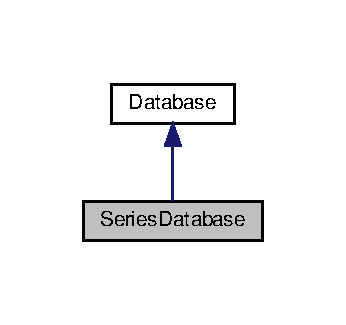
\includegraphics[width=166pt]{classSeriesDatabase__inherit__graph}
\end{center}
\end{figure}


Collaboration diagram for Series\+Database\+:\nopagebreak
\begin{figure}[H]
\begin{center}
\leavevmode
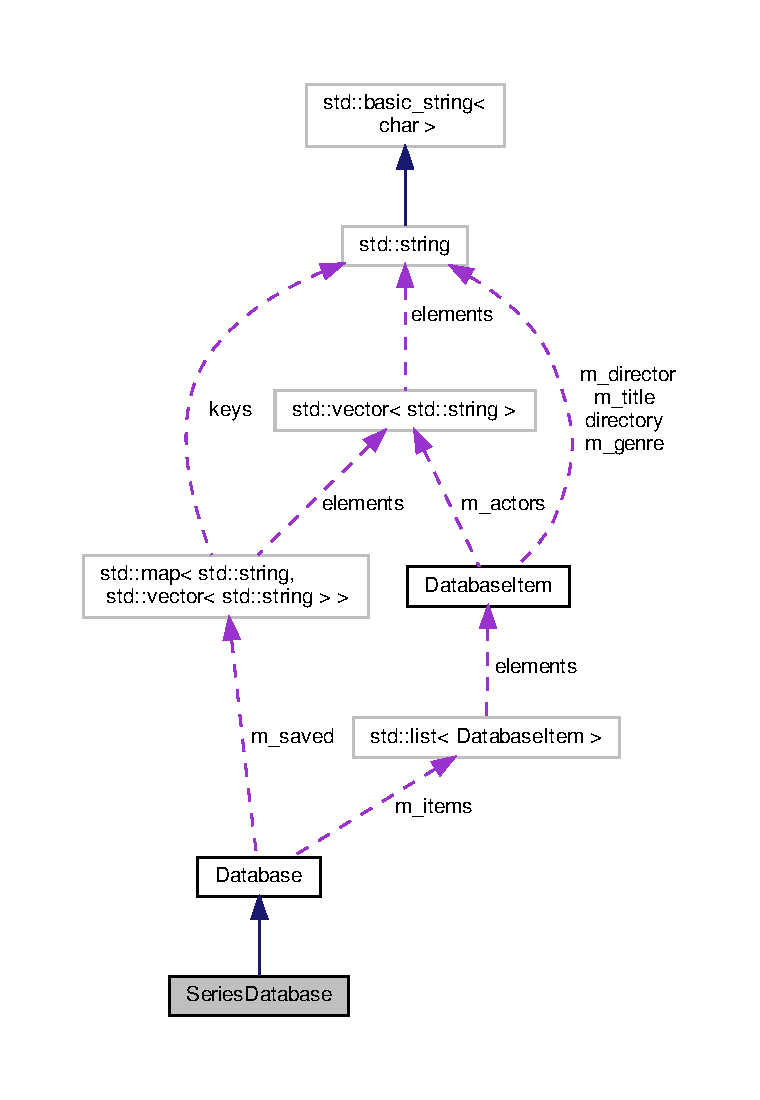
\includegraphics[width=350pt]{classSeriesDatabase__coll__graph}
\end{center}
\end{figure}
\subsection*{Public Member Functions}
\begin{DoxyCompactItemize}
\item 
void \hyperlink{classSeriesDatabase_a0ba159b6d52a3cfa07135c7d8b37ef76}{sync\+Local\+Database} () override
\begin{DoxyCompactList}\small\item\em Sync info from json file and saves it to a list of database objects. \end{DoxyCompactList}\item 
void \hyperlink{classSeriesDatabase_a7591f89ab256d9f5a41235f5552e4e23}{push\+Item} (const \hyperlink{classDatabaseItem}{Database\+Item} \&m\+\_\+item) override
\begin{DoxyCompactList}\small\item\em Implementation for virtual member of \hyperlink{Database_8h_source}{Database.\+h} Method that uploads the requested database item. \end{DoxyCompactList}\item 
\hyperlink{classDatabaseItem}{Database\+Item} \hyperlink{classSeriesDatabase_af5303a723910395b31f2e01088de9130}{fetch\+Item} (const std\+::string \&title) override
\begin{DoxyCompactList}\small\item\em Implementation for virtual member of \hyperlink{Database_8h_source}{Database.\+h} Method that fetches the requested database item. \end{DoxyCompactList}\item 
long \hyperlink{classSeriesDatabase_af5fe5a423303eff4489a7679907ef994}{get\+Number\+Of\+Item} () override
\begin{DoxyCompactList}\small\item\em Implementation for virtual member of \hyperlink{Database_8h_source}{Database.\+h} Method that return the size of the database. \end{DoxyCompactList}\item 
void \hyperlink{classSeriesDatabase_a863a35987b5a4de15a121b8b4358e353}{purge\+Item} (\hyperlink{classDatabaseItem}{Database\+Item} item) override
\begin{DoxyCompactList}\small\item\em Implementation for virtual member of \hyperlink{Database_8h_source}{Database.\+h} Method that deletes the requested database item. \end{DoxyCompactList}\item 
void \hyperlink{classSeriesDatabase_ae2bf5323216e0043292494d3f0ac978c}{print\+All} () override
\begin{DoxyCompactList}\small\item\em Implementation for virtual member of \hyperlink{Database_8h_source}{Database.\+h} Method that prints the entire database content. \end{DoxyCompactList}\end{DoxyCompactItemize}
\subsection*{Protected Attributes}
\begin{DoxyCompactItemize}
\item 
std\+::list$<$ \hyperlink{classDatabaseItem}{Database\+Item} $>$ \hyperlink{classDatabase_a5a4ac1f3bf0f5fd77a696174ad9e5c45}{m\+\_\+items}
\begin{DoxyCompactList}\small\item\em A protected list of Database\+Items. \end{DoxyCompactList}\item 
std\+::map$<$ std\+::string, std\+::vector$<$ std\+::string $>$ $>$ \hyperlink{classDatabase_a9f87cbe5a1be71d541083dffa8d8c9ad}{m\+\_\+saved}
\begin{DoxyCompactList}\small\item\em A protected vector of strings with info for the Database\+Items. \end{DoxyCompactList}\item 
std\+::mutex \hyperlink{classDatabase_a7f55f3a5d93c9694ee4f08a2f2135b1d}{m\+\_\+lock}
\begin{DoxyCompactList}\small\item\em A protected mutex for threadsafe r/w of Database\+Items. \end{DoxyCompactList}\item 
std\+::condition\+\_\+variable \hyperlink{classDatabase_a2ad8bf38964b3e18a0e168437acbdb27}{m\+\_\+empty\+List}
\begin{DoxyCompactList}\small\item\em A protected condittion variable for the mutex and \hyperlink{classDatabase}{Database} list. \end{DoxyCompactList}\end{DoxyCompactItemize}


\subsection{Member Function Documentation}
\mbox{\Hypertarget{classSeriesDatabase_af5303a723910395b31f2e01088de9130}\label{classSeriesDatabase_af5303a723910395b31f2e01088de9130}} 
\index{Series\+Database@{Series\+Database}!fetch\+Item@{fetch\+Item}}
\index{fetch\+Item@{fetch\+Item}!Series\+Database@{Series\+Database}}
\subsubsection{\texorpdfstring{fetch\+Item()}{fetchItem()}}
{\footnotesize\ttfamily \hyperlink{classDatabaseItem}{Database\+Item} Series\+Database\+::fetch\+Item (\begin{DoxyParamCaption}\item[{const std\+::string \&}]{title }\end{DoxyParamCaption})\hspace{0.3cm}{\ttfamily [inline]}, {\ttfamily [override]}, {\ttfamily [virtual]}}



Implementation for virtual member of \hyperlink{Database_8h_source}{Database.\+h} Method that fetches the requested database item. 

A const reference to a title

\begin{DoxyReturn}{Returns}
The requested \hyperlink{classDatabaseItem}{Database\+Item}
\end{DoxyReturn}


Reimplemented from \hyperlink{classDatabase_a40254eec69c7d7cc15da24a9f0b072b3}{Database}.

\mbox{\Hypertarget{classSeriesDatabase_af5fe5a423303eff4489a7679907ef994}\label{classSeriesDatabase_af5fe5a423303eff4489a7679907ef994}} 
\index{Series\+Database@{Series\+Database}!get\+Number\+Of\+Item@{get\+Number\+Of\+Item}}
\index{get\+Number\+Of\+Item@{get\+Number\+Of\+Item}!Series\+Database@{Series\+Database}}
\subsubsection{\texorpdfstring{get\+Number\+Of\+Item()}{getNumberOfItem()}}
{\footnotesize\ttfamily long Series\+Database\+::get\+Number\+Of\+Item (\begin{DoxyParamCaption}{ }\end{DoxyParamCaption})\hspace{0.3cm}{\ttfamily [inline]}, {\ttfamily [override]}, {\ttfamily [virtual]}}



Implementation for virtual member of \hyperlink{Database_8h_source}{Database.\+h} Method that return the size of the database. 

\begin{DoxyReturn}{Returns}
Size of the database (long).
\end{DoxyReturn}


Reimplemented from \hyperlink{classDatabase_a230225cb341eb23a99a83ef3d1abae53}{Database}.

\mbox{\Hypertarget{classSeriesDatabase_ae2bf5323216e0043292494d3f0ac978c}\label{classSeriesDatabase_ae2bf5323216e0043292494d3f0ac978c}} 
\index{Series\+Database@{Series\+Database}!print\+All@{print\+All}}
\index{print\+All@{print\+All}!Series\+Database@{Series\+Database}}
\subsubsection{\texorpdfstring{print\+All()}{printAll()}}
{\footnotesize\ttfamily void Series\+Database\+::print\+All (\begin{DoxyParamCaption}{ }\end{DoxyParamCaption})\hspace{0.3cm}{\ttfamily [inline]}, {\ttfamily [override]}, {\ttfamily [virtual]}}



Implementation for virtual member of \hyperlink{Database_8h_source}{Database.\+h} Method that prints the entire database content. 



Reimplemented from \hyperlink{classDatabase_afa345da530fd5c8dfe0c978917cd6049}{Database}.

\mbox{\Hypertarget{classSeriesDatabase_a863a35987b5a4de15a121b8b4358e353}\label{classSeriesDatabase_a863a35987b5a4de15a121b8b4358e353}} 
\index{Series\+Database@{Series\+Database}!purge\+Item@{purge\+Item}}
\index{purge\+Item@{purge\+Item}!Series\+Database@{Series\+Database}}
\subsubsection{\texorpdfstring{purge\+Item()}{purgeItem()}}
{\footnotesize\ttfamily void Series\+Database\+::purge\+Item (\begin{DoxyParamCaption}\item[{\hyperlink{classDatabaseItem}{Database\+Item}}]{item }\end{DoxyParamCaption})\hspace{0.3cm}{\ttfamily [inline]}, {\ttfamily [override]}, {\ttfamily [virtual]}}



Implementation for virtual member of \hyperlink{Database_8h_source}{Database.\+h} Method that deletes the requested database item. 

A const reference to a database item

Reimplemented from \hyperlink{classDatabase_a8f47437526eeec631f1328fab9bbbc75}{Database}.

\mbox{\Hypertarget{classSeriesDatabase_a7591f89ab256d9f5a41235f5552e4e23}\label{classSeriesDatabase_a7591f89ab256d9f5a41235f5552e4e23}} 
\index{Series\+Database@{Series\+Database}!push\+Item@{push\+Item}}
\index{push\+Item@{push\+Item}!Series\+Database@{Series\+Database}}
\subsubsection{\texorpdfstring{push\+Item()}{pushItem()}}
{\footnotesize\ttfamily void Series\+Database\+::push\+Item (\begin{DoxyParamCaption}\item[{const \hyperlink{classDatabaseItem}{Database\+Item} \&}]{m\+\_\+item }\end{DoxyParamCaption})\hspace{0.3cm}{\ttfamily [inline]}, {\ttfamily [override]}, {\ttfamily [virtual]}}



Implementation for virtual member of \hyperlink{Database_8h_source}{Database.\+h} Method that uploads the requested database item. 

A const reference to a database item

\begin{DoxyReturn}{Returns}

\end{DoxyReturn}


Reimplemented from \hyperlink{classDatabase_a80fa14ab9f4deadc9a2ab7493f1919a4}{Database}.

Here is the caller graph for this function\+:\nopagebreak
\begin{figure}[H]
\begin{center}
\leavevmode
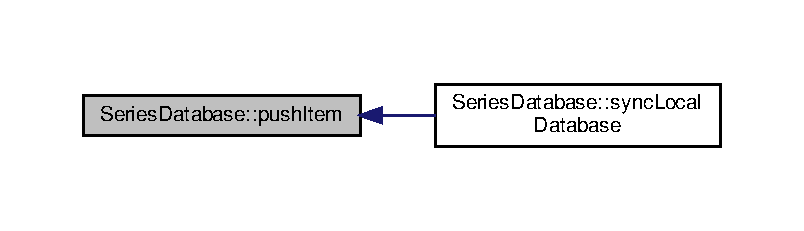
\includegraphics[width=350pt]{classSeriesDatabase_a7591f89ab256d9f5a41235f5552e4e23_icgraph}
\end{center}
\end{figure}
\mbox{\Hypertarget{classSeriesDatabase_a0ba159b6d52a3cfa07135c7d8b37ef76}\label{classSeriesDatabase_a0ba159b6d52a3cfa07135c7d8b37ef76}} 
\index{Series\+Database@{Series\+Database}!sync\+Local\+Database@{sync\+Local\+Database}}
\index{sync\+Local\+Database@{sync\+Local\+Database}!Series\+Database@{Series\+Database}}
\subsubsection{\texorpdfstring{sync\+Local\+Database()}{syncLocalDatabase()}}
{\footnotesize\ttfamily void Series\+Database\+::sync\+Local\+Database (\begin{DoxyParamCaption}{ }\end{DoxyParamCaption})\hspace{0.3cm}{\ttfamily [inline]}, {\ttfamily [override]}, {\ttfamily [virtual]}}



Sync info from json file and saves it to a list of database objects. 

Database\+::sync\+Database() 

Reimplemented from \hyperlink{classDatabase_a14d24487b4ea3b50097b9ac0f2b3f317}{Database}.

Here is the call graph for this function\+:\nopagebreak
\begin{figure}[H]
\begin{center}
\leavevmode
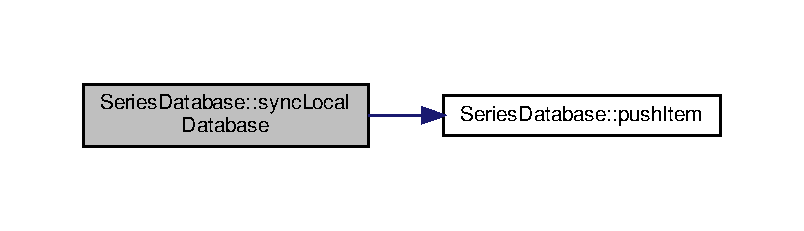
\includegraphics[width=350pt]{classSeriesDatabase_a0ba159b6d52a3cfa07135c7d8b37ef76_cgraph}
\end{center}
\end{figure}


\subsection{Member Data Documentation}
\mbox{\Hypertarget{classDatabase_a2ad8bf38964b3e18a0e168437acbdb27}\label{classDatabase_a2ad8bf38964b3e18a0e168437acbdb27}} 
\index{Series\+Database@{Series\+Database}!m\+\_\+empty\+List@{m\+\_\+empty\+List}}
\index{m\+\_\+empty\+List@{m\+\_\+empty\+List}!Series\+Database@{Series\+Database}}
\subsubsection{\texorpdfstring{m\+\_\+empty\+List}{m\_emptyList}}
{\footnotesize\ttfamily std\+::condition\+\_\+variable Database\+::m\+\_\+empty\+List\hspace{0.3cm}{\ttfamily [protected]}, {\ttfamily [inherited]}}



A protected condittion variable for the mutex and \hyperlink{classDatabase}{Database} list. 

\mbox{\Hypertarget{classDatabase_a5a4ac1f3bf0f5fd77a696174ad9e5c45}\label{classDatabase_a5a4ac1f3bf0f5fd77a696174ad9e5c45}} 
\index{Series\+Database@{Series\+Database}!m\+\_\+items@{m\+\_\+items}}
\index{m\+\_\+items@{m\+\_\+items}!Series\+Database@{Series\+Database}}
\subsubsection{\texorpdfstring{m\+\_\+items}{m\_items}}
{\footnotesize\ttfamily std\+::list$<$\hyperlink{classDatabaseItem}{Database\+Item}$>$ Database\+::m\+\_\+items\hspace{0.3cm}{\ttfamily [protected]}, {\ttfamily [inherited]}}



A protected list of Database\+Items. 

\mbox{\Hypertarget{classDatabase_a7f55f3a5d93c9694ee4f08a2f2135b1d}\label{classDatabase_a7f55f3a5d93c9694ee4f08a2f2135b1d}} 
\index{Series\+Database@{Series\+Database}!m\+\_\+lock@{m\+\_\+lock}}
\index{m\+\_\+lock@{m\+\_\+lock}!Series\+Database@{Series\+Database}}
\subsubsection{\texorpdfstring{m\+\_\+lock}{m\_lock}}
{\footnotesize\ttfamily std\+::mutex Database\+::m\+\_\+lock\hspace{0.3cm}{\ttfamily [mutable]}, {\ttfamily [protected]}, {\ttfamily [inherited]}}



A protected mutex for threadsafe r/w of Database\+Items. 

\mbox{\Hypertarget{classDatabase_a9f87cbe5a1be71d541083dffa8d8c9ad}\label{classDatabase_a9f87cbe5a1be71d541083dffa8d8c9ad}} 
\index{Series\+Database@{Series\+Database}!m\+\_\+saved@{m\+\_\+saved}}
\index{m\+\_\+saved@{m\+\_\+saved}!Series\+Database@{Series\+Database}}
\subsubsection{\texorpdfstring{m\+\_\+saved}{m\_saved}}
{\footnotesize\ttfamily std\+::map$<$std\+::string, std\+::vector$<$std\+::string$>$ $>$ Database\+::m\+\_\+saved\hspace{0.3cm}{\ttfamily [protected]}, {\ttfamily [inherited]}}



A protected vector of strings with info for the Database\+Items. 



The documentation for this class was generated from the following file\+:\begin{DoxyCompactItemize}
\item 
inc/database/Series\+Database.\+h\end{DoxyCompactItemize}

\hypertarget{classSshConnector}{}\section{Ssh\+Connector Class Reference}
\label{classSshConnector}\index{Ssh\+Connector@{Ssh\+Connector}}


Inheritance diagram for Ssh\+Connector\+:\nopagebreak
\begin{figure}[H]
\begin{center}
\leavevmode
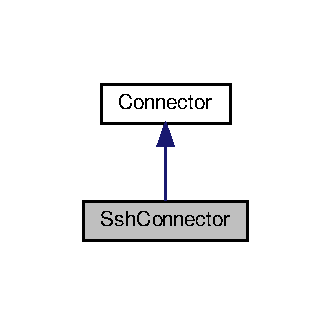
\includegraphics[width=159pt]{classSshConnector__inherit__graph}
\end{center}
\end{figure}


Collaboration diagram for Ssh\+Connector\+:\nopagebreak
\begin{figure}[H]
\begin{center}
\leavevmode
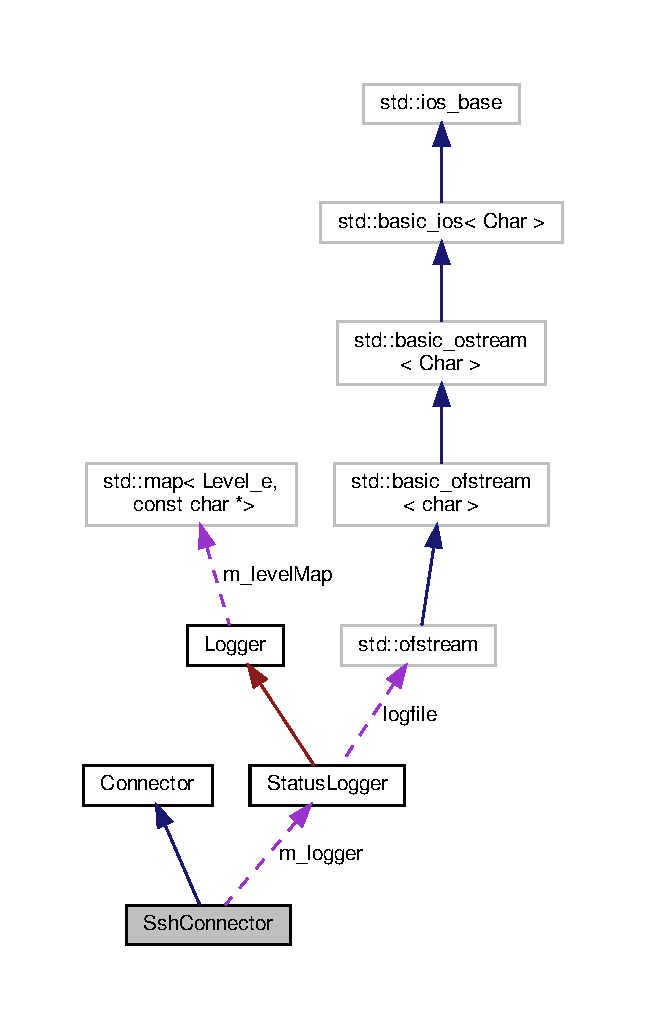
\includegraphics[width=310pt]{classSshConnector__coll__graph}
\end{center}
\end{figure}
\subsection*{Public Member Functions}
\begin{DoxyCompactItemize}
\item 
\mbox{\Hypertarget{classSshConnector_aeb1020e975caa51b24b49180362bf916}\label{classSshConnector_aeb1020e975caa51b24b49180362bf916}} 
\hyperlink{classConnectionStream}{Connection\+Stream} $\ast$ {\bfseries connect} (uint16\+\_\+t port, std\+::string server) override
\item 
\mbox{\Hypertarget{classSshConnector_a54af419fdb2ec6ffa7aad86b294da681}\label{classSshConnector_a54af419fdb2ec6ffa7aad86b294da681}} 
void {\bfseries disconnect} () override
\end{DoxyCompactItemize}
\subsection*{Public Attributes}
\begin{DoxyCompactItemize}
\item 
\mbox{\Hypertarget{classSshConnector_ac31406197a9f7313f07945d85939ea31}\label{classSshConnector_ac31406197a9f7313f07945d85939ea31}} 
bool {\bfseries m\+\_\+currently\+Connected}
\end{DoxyCompactItemize}
\subsection*{Protected Member Functions}
\begin{DoxyCompactItemize}
\item 
\mbox{\Hypertarget{classSshConnector_a1d56102ea6b4fa9b632b4a09a82b1384}\label{classSshConnector_a1d56102ea6b4fa9b632b4a09a82b1384}} 
int {\bfseries resolve\+Host} (ssh\+\_\+session session) override
\end{DoxyCompactItemize}
\subsection*{Private Attributes}
\begin{DoxyCompactItemize}
\item 
\mbox{\Hypertarget{classSshConnector_a50ffdb805cbc4b2cafb11d83b3858095}\label{classSshConnector_a50ffdb805cbc4b2cafb11d83b3858095}} 
\hyperlink{classStatusLogger}{Status\+Logger} $\ast$ {\bfseries m\+\_\+logger}
\item 
\mbox{\Hypertarget{classSshConnector_ae66617dc5bb646d9de70adfae28eccd5}\label{classSshConnector_ae66617dc5bb646d9de70adfae28eccd5}} 
ssh\+\_\+session {\bfseries m\+\_\+session} \{ \}
\item 
\mbox{\Hypertarget{classSshConnector_a24af12d393d809a47c750ad3be02bbad}\label{classSshConnector_a24af12d393d809a47c750ad3be02bbad}} 
unsigned char $\ast$ {\bfseries m\+\_\+hash} = nullptr
\item 
\mbox{\Hypertarget{classSshConnector_a7d02d2d3bfad85572058d354d6fc59c9}\label{classSshConnector_a7d02d2d3bfad85572058d354d6fc59c9}} 
char $\ast$ {\bfseries m\+\_\+hexa} \{ \}
\end{DoxyCompactItemize}


The documentation for this class was generated from the following files\+:\begin{DoxyCompactItemize}
\item 
inc/Ssh\+Connector.\+h\item 
src/Ssh\+Connector.\+cpp\end{DoxyCompactItemize}

\hypertarget{classStatusLogger}{}\section{Status\+Logger Class Reference}
\label{classStatusLogger}\index{Status\+Logger@{Status\+Logger}}


Inheritance diagram for Status\+Logger\+:\nopagebreak
\begin{figure}[H]
\begin{center}
\leavevmode
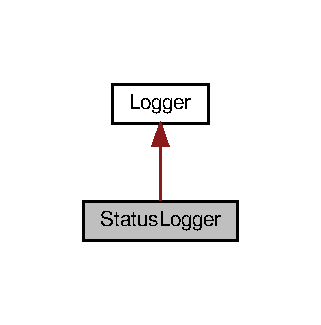
\includegraphics[width=154pt]{classStatusLogger__inherit__graph}
\end{center}
\end{figure}


Collaboration diagram for Status\+Logger\+:\nopagebreak
\begin{figure}[H]
\begin{center}
\leavevmode
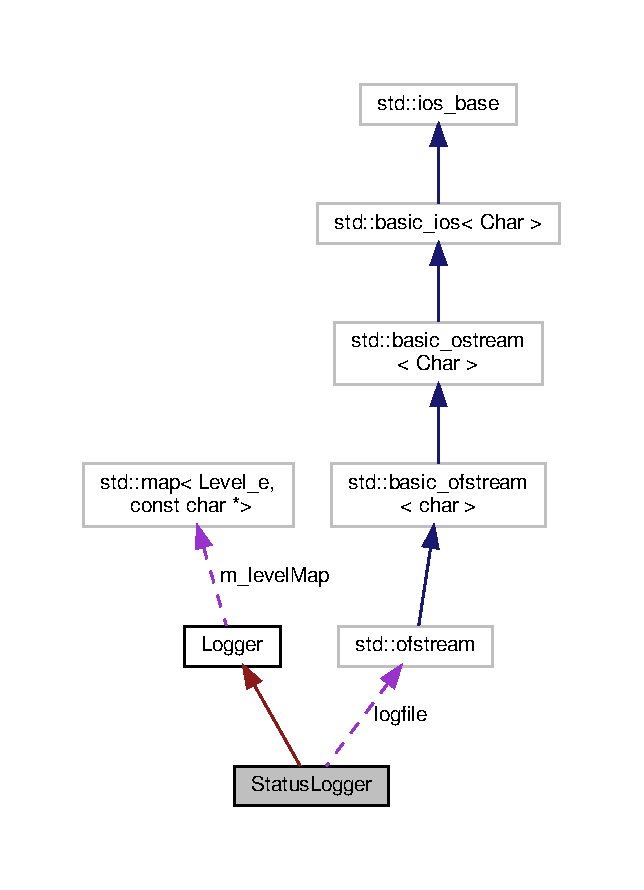
\includegraphics[width=309pt]{classStatusLogger__coll__graph}
\end{center}
\end{figure}
\subsection*{Public Member Functions}
\begin{DoxyCompactItemize}
\item 
\mbox{\Hypertarget{classStatusLogger_ab1b31ad74fac19bddddb34949b3eb0a1}\label{classStatusLogger_ab1b31ad74fac19bddddb34949b3eb0a1}} 
void {\bfseries T\+R\+A\+CE} (Level\+\_\+e level, std\+::string message, std\+::string error\+Code) override
\item 
\mbox{\Hypertarget{classStatusLogger_a9cd751e71f814914694e9c4ed39df0f9}\label{classStatusLogger_a9cd751e71f814914694e9c4ed39df0f9}} 
void {\bfseries T\+R\+A\+CE} (Level\+\_\+e level, std\+::string message) override
\end{DoxyCompactItemize}
\subsection*{Private Types}
\begin{DoxyCompactItemize}
\item 
\mbox{\Hypertarget{classLogger_aa1875ace78bce45b33f84d7f5de7790d}\label{classLogger_aa1875ace78bce45b33f84d7f5de7790d}} 
enum {\bfseries Level\+\_\+e} \{ {\bfseries I\+N\+FO} = 0, 
{\bfseries E\+RR} = 1, 
{\bfseries W\+A\+RN} = 2
 \}
\end{DoxyCompactItemize}
\subsection*{Private Member Functions}
\begin{DoxyCompactItemize}
\item 
\mbox{\Hypertarget{classStatusLogger_a68965a0651d02b978a389d34d5c1fec3}\label{classStatusLogger_a68965a0651d02b978a389d34d5c1fec3}} 
std\+::string {\bfseries get\+Filename} ()
\item 
\mbox{\Hypertarget{classStatusLogger_aa48b918db673aaeb1c663b7e0cad6655}\label{classStatusLogger_aa48b918db673aaeb1c663b7e0cad6655}} 
std\+::string {\bfseries Get\+Current\+Working\+Dir} ()
\item 
\mbox{\Hypertarget{classStatusLogger_aa110fa026ef5e5a6a5b250623c73faa6}\label{classStatusLogger_aa110fa026ef5e5a6a5b250623c73faa6}} 
void {\bfseries write} (Level\+\_\+e level, std\+::string \&output)
\item 
\mbox{\Hypertarget{classLogger_ac05df84a2b15ca6e1b3b6119a3b7a32c}\label{classLogger_ac05df84a2b15ca6e1b3b6119a3b7a32c}} 
std\+::string {\bfseries get\+Date} ()
\item 
\mbox{\Hypertarget{classLogger_af6e809c7f6fe8d2f829ce0d6a760e0ce}\label{classLogger_af6e809c7f6fe8d2f829ce0d6a760e0ce}} 
std\+::string {\bfseries get\+Time} ()
\item 
\mbox{\Hypertarget{classLogger_a8416f3e0b6fa98d42ca890c0577dff34}\label{classLogger_a8416f3e0b6fa98d42ca890c0577dff34}} 
{\footnotesize template$<$typename T $>$ }\\\hyperlink{structLogger_1_1map__init__helper}{map\+\_\+init\+\_\+helper}$<$ T $>$ {\bfseries map\+\_\+init} (T \&item)
\end{DoxyCompactItemize}
\subsection*{Private Attributes}
\begin{DoxyCompactItemize}
\item 
\mbox{\Hypertarget{classStatusLogger_a166f1d6b8016d9c203dd98f16cc488fc}\label{classStatusLogger_a166f1d6b8016d9c203dd98f16cc488fc}} 
std\+::ofstream {\bfseries logfile}
\item 
\mbox{\Hypertarget{classLogger_a5e3acb7eae07a5cee57d28711ce45413}\label{classLogger_a5e3acb7eae07a5cee57d28711ce45413}} 
std\+::map$<$ Level\+\_\+e, const char $\ast$ $>$ {\bfseries m\+\_\+level\+Map}
\end{DoxyCompactItemize}
\subsection*{Static Private Attributes}
\begin{DoxyCompactItemize}
\item 
\mbox{\Hypertarget{classLogger_ade70cee1c967259b5dc2448424c7df68}\label{classLogger_ade70cee1c967259b5dc2448424c7df68}} 
static enum Logger\+::\+Level\+\_\+e {\bfseries level}
\end{DoxyCompactItemize}


The documentation for this class was generated from the following file\+:\begin{DoxyCompactItemize}
\item 
inc/Status\+Logger.\+h\end{DoxyCompactItemize}

\hypertarget{classSubject}{}\section{Subject Class Reference}
\label{classSubject}\index{Subject@{Subject}}


{\ttfamily \#include $<$Subject.\+h$>$}



Inheritance diagram for Subject\+:\nopagebreak
\begin{figure}[H]
\begin{center}
\leavevmode
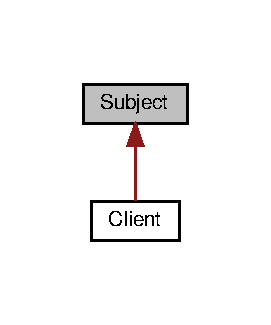
\includegraphics[width=130pt]{classSubject__inherit__graph}
\end{center}
\end{figure}
\subsection*{Public Member Functions}
\begin{DoxyCompactItemize}
\item 
virtual void \hyperlink{classSubject_ae3f8d320b19b7d0fe695a3b4e7660002}{register\+Observer} (\hyperlink{classObserver}{Observer} $\ast$observer)=0
\item 
virtual void \hyperlink{classSubject_a86699df0364a9091d1887f344255e9ff}{remove\+Observer} (\hyperlink{classObserver}{Observer} $\ast$observer)=0
\item 
virtual void \hyperlink{classSubject_ad779772e3bcf5b3bd8f7a96b10531920}{notify\+Observers} (\hyperlink{classRequest}{Request} \&)=0
\end{DoxyCompactItemize}


\subsection{Detailed Description}
Interface for the \hyperlink{classSubject}{Subject} 

\subsection{Member Function Documentation}
\mbox{\Hypertarget{classSubject_ad779772e3bcf5b3bd8f7a96b10531920}\label{classSubject_ad779772e3bcf5b3bd8f7a96b10531920}} 
\index{Subject@{Subject}!notify\+Observers@{notify\+Observers}}
\index{notify\+Observers@{notify\+Observers}!Subject@{Subject}}
\subsubsection{\texorpdfstring{notify\+Observers()}{notifyObservers()}}
{\footnotesize\ttfamily virtual void Subject\+::notify\+Observers (\begin{DoxyParamCaption}\item[{\hyperlink{classRequest}{Request} \&}]{ }\end{DoxyParamCaption})\hspace{0.3cm}{\ttfamily [pure virtual]}}

Notify all the registered observers when a change happens 

Implemented in \hyperlink{classClient_a2fb08fe51afa68997faa22474e114771}{Client}.

\mbox{\Hypertarget{classSubject_ae3f8d320b19b7d0fe695a3b4e7660002}\label{classSubject_ae3f8d320b19b7d0fe695a3b4e7660002}} 
\index{Subject@{Subject}!register\+Observer@{register\+Observer}}
\index{register\+Observer@{register\+Observer}!Subject@{Subject}}
\subsubsection{\texorpdfstring{register\+Observer()}{registerObserver()}}
{\footnotesize\ttfamily virtual void Subject\+::register\+Observer (\begin{DoxyParamCaption}\item[{\hyperlink{classObserver}{Observer} $\ast$}]{observer }\end{DoxyParamCaption})\hspace{0.3cm}{\ttfamily [pure virtual]}}

Register an observer 
\begin{DoxyParams}{Parameters}
{\em observer} & the observer object to be registered \\
\hline
\end{DoxyParams}


Implemented in \hyperlink{classClient_a1426f0582287f6c583d8681e540059ab}{Client}.

\mbox{\Hypertarget{classSubject_a86699df0364a9091d1887f344255e9ff}\label{classSubject_a86699df0364a9091d1887f344255e9ff}} 
\index{Subject@{Subject}!remove\+Observer@{remove\+Observer}}
\index{remove\+Observer@{remove\+Observer}!Subject@{Subject}}
\subsubsection{\texorpdfstring{remove\+Observer()}{removeObserver()}}
{\footnotesize\ttfamily virtual void Subject\+::remove\+Observer (\begin{DoxyParamCaption}\item[{\hyperlink{classObserver}{Observer} $\ast$}]{observer }\end{DoxyParamCaption})\hspace{0.3cm}{\ttfamily [pure virtual]}}

Unregister an observer 
\begin{DoxyParams}{Parameters}
{\em observer} & the observer object to be unregistered \\
\hline
\end{DoxyParams}


Implemented in \hyperlink{classClient_abfce703b679961b961ff24bbfc532ce4}{Client}.



The documentation for this class was generated from the following file\+:\begin{DoxyCompactItemize}
\item 
inc/ifc/Subject.\+h\end{DoxyCompactItemize}

%--- End generated contents ---

% Index
\backmatter
\newpage
\phantomsection
\clearemptydoublepage
\addcontentsline{toc}{chapter}{Index}
\printindex

\end{document}
